\chapter{Pulsar Wind Nebulae} \label{sec:01_PWN_chapter}

The last couple of centuries have seen astronomy being turned from a navigators map into a diverse field full of extremes. High-energy astrophysics is one of these extremes and investigates cosmic rays and gamma rays released by the most energetic events in the Universe. One source of cosmic rays are PWNe, which can be seen across the electromagnetic spectrum from radio waves up to gamma rays. The linking of fundamental physics to gamma-ray observations can provide a window into the understanding of PWNe.
This chapter is divided as follows: \autoref{sec:01_PWN} discusses the structure and evolution of PWN before highlighting the $\TeV$ PWN \mbox{HESS\,J1825-137} and nearby northern source \mbox{HESS\,J1826-130}. Cosmic rays are then investigated in further detail in \autoref{sec:01_cosmic_rays} before describing the pathways of gamma ray production by cosmic rays in \autoref{sec:chapter1_non_thermal_emission}.

\section{Pulsar Wind Nebulae} \label{sec:01_PWN}

\subsection{Neutron Stars/ Pulsars} \label{sec:01_PWN_pulsar}

\begin{wrapfigure}{R}{0.5\textwidth}
	\centering
	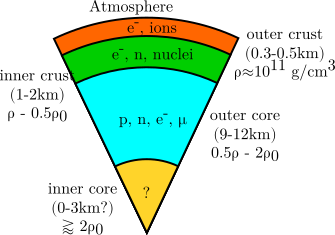
\includegraphics[width=0.5\textwidth]{04_Introduction/Images/pulsar_wind_nebula/pulsar_structure.png}
	\caption{The neutron star/pulsar structure is composed of an inner \& outer core, inner \& outer crust and an atmosphere \citep{2007ASSL..326.....H}.}
	\label{fig:chapter1_pulsar_structure}
\end{wrapfigure}

In 1967 Jocelyn Bell and Antony Hewish observed a series of radio pulses every $1.33\,\si{\second}$ originating from the same location in the night sky. The object was label LGM-1, short for `little green men', and became the first known neutron star/pulsar. First proposed by Walter Baade and Fritz Zwicky in the 1930's \citep{1934PhRv...46...76B}, neutron stars are the rotating, highly dense, magnetised remnants of massive stars that emit beams of photons from its magnetic poles. The magnetic and rotational axes do not necessarily align and the beams of photons rotate around the neutron star. A neutron star is a pulsar when the beam of light points in the direction of earth, forming the characteristic pulse.
\newpar
Neutron stars are formed during a supernova when a massive star ($\gtrsim 8~M_\odot$) can no longer support the immense gravitational pressure due to accumulation of iron in the core and undergoes core collapse. Gravitational pressure overcomes electron-degeneracy pressure, forcing electrons and protons in the core to combine to form neutrons. At this point, neutron-degeneracy and the strong force prevents further collapse and the neutron star is created. If the neutron star mass exceeds the Tolman–Oppenheimer–Volkoff limit ($1.5-3~M_\odot$), further collapse can result in a black hole \citep{1996A&A...305..871B, 2015SSRv..188..187S}.
\newpar
Neutron stars have a mass of $1-3~M_\odot$, average density $\rho_0=2.8\times 10^{14}\si{\gram\per\centi\meter\cubed}$ (nuclear saturated mass density) and a radius $10-15\,\si{\kilo\meter}$ which is subdivided into the following layers (see \autoref{fig:chapter1_pulsar_structure}) \citep{2007ASSL..326.....H}: the \textbf{atmosphere} consists of a thin layer of plasma (electrons and light nuclei) up to $10\,\cm$ thick with temperature around $10^5-10^6\,\si{\kelvin}$ \citep{2002nsps.conf..263Z}. The magnetic field of $10^{11}-10^{14}\,\si{G}$ controls the dynamics of the atmosphere. Ions and electrons make up the \textbf{outer crust} in a layer of $0.3-0.5\,\km$ thickness of density $\rho=4\times 10^{11}\,\si{\gram\per\centi\meter\cubed}$. Just below the atmosphere, a thin non-degenerate electron gas forms the edge of the outer crust. This gives way to a liquid/solid crust where nuclei undergo electron capture forming neutrons. The \textbf{inner crust} is around $1\,\km$ thick, has average density of $0.3-0.5\rho_0$ and is composed of electrons, neutrons and neutron-rich nuclei. Both the inner and outer crust have been postulated to contain `nuclear pasta', degenerate matter where neutrons and electrons arrange themselves into complex structures \citep{PhysRevC.88.065807}. The \textbf{outer core} is the thickest part of the neutron star at around $9-12\,\km$ thick and has density $0.5-2.0\rho_0$. The \textbf{inner core} exists at the centre of the more massive neutron stars with conditions so extreme, it has been postulated that protons and neutrons break up into their constituent quarks \citep{2007ASSL..326.....H}.
\begin{figure}[b!]
	\centering
	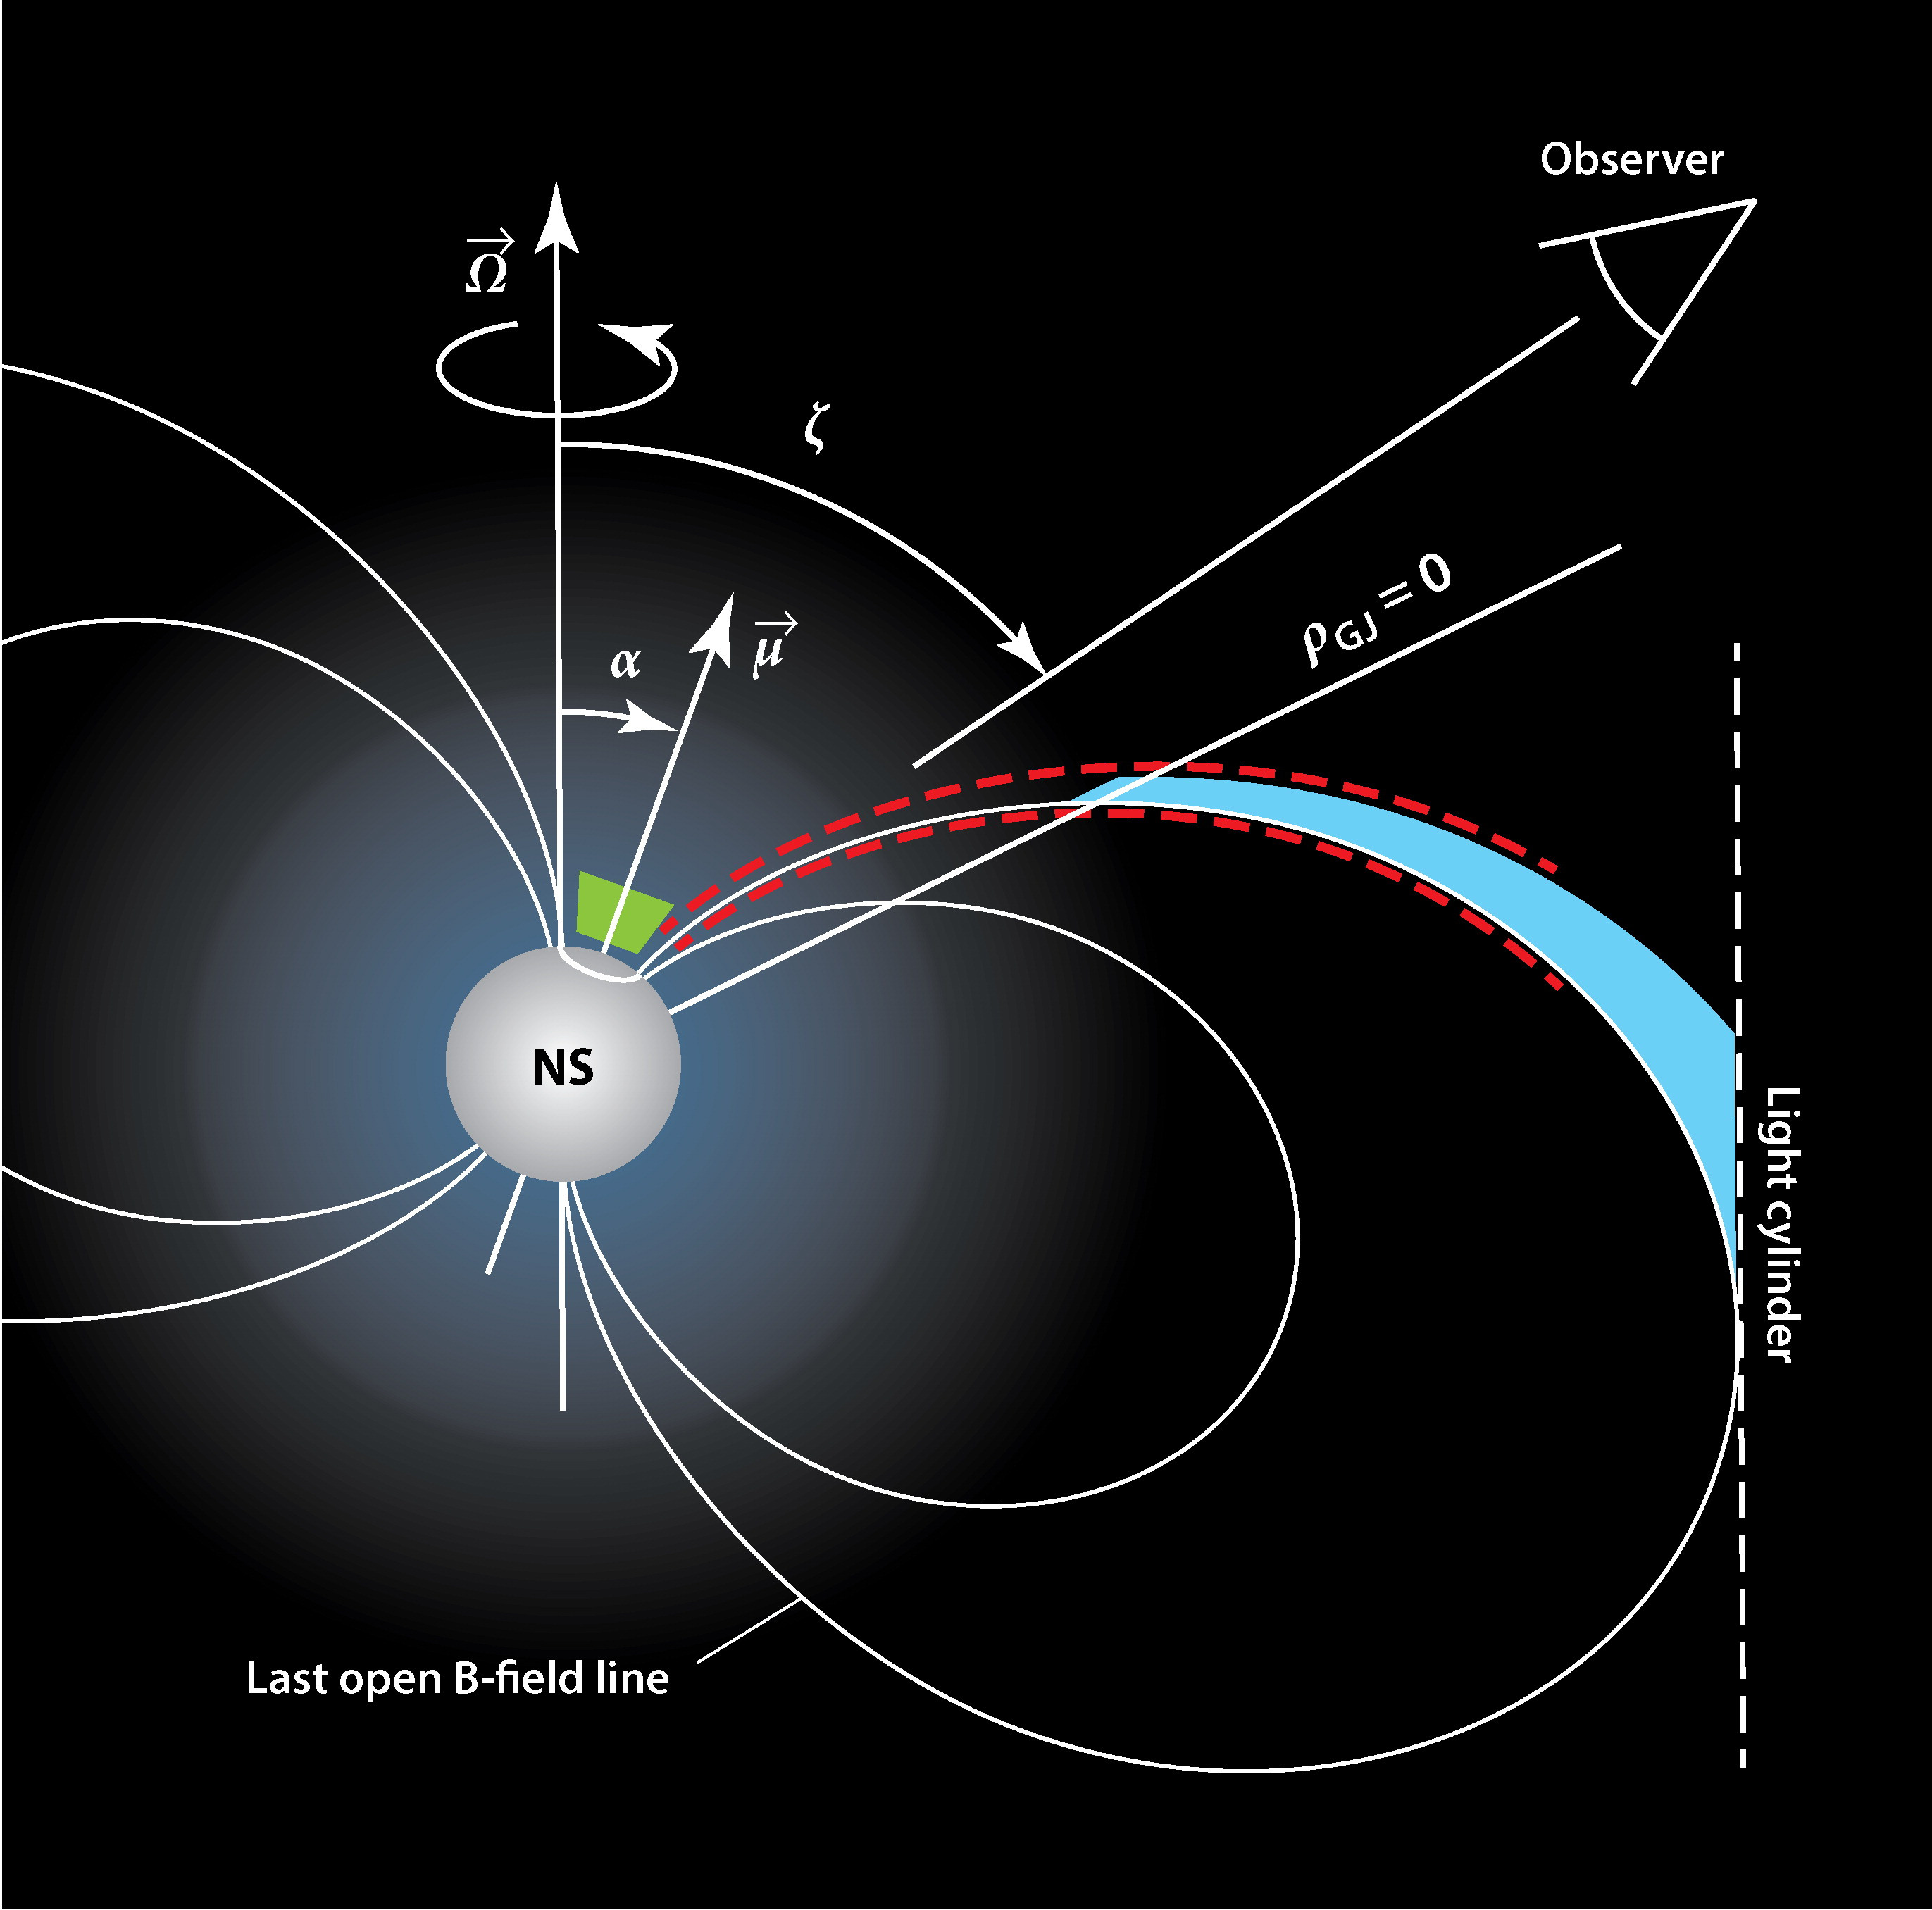
\includegraphics[width=0.7\textwidth]{04_Introduction/Images/pulsar_wind_nebula/pulsar.jpeg}
	\caption{Magnetosphere structure of a pulsar with spin velocity $\vec{\Omega}$ at angle $\alpha$ to the magnetic field axis and angle $\zeta$ to the observer. The acceleration site for the polar cap model and outer gap model is shown in green and blue respectively while the site for the slot gap model is enclosed by the red-dashed lines. Image courtesy of \cite{2014ARA&A..52..211C}.}
	\label{fig:chapter1_magnetosphere_structure}
\end{figure}
\newpar
After core collapse, pulsars retain the majority of a progenitor star's angular momentum ($L=m\omega r$; $m$ is the pulsar mass, $\omega$ is the spin velocity and $r$ is the pulsar radius), leading to the pulsar spinning rapidly on its axis. Based on the assumption that the magnetic flux of the progenitor star is conserved, \cite{1964ApJ...140.1309W} proposed that the pulsar's magnetic field could be as strong as $10^{14}-10^{16}\,\si{G}$. The rotation coupled with the magnetic field, $\vec{B}$, generates an electric field given by:

\begin{equation}
    \begin{aligned}
    \vec{E} &= - \vec{v} \times \vec{B}\text{ ,}
    \end{aligned}
\end{equation}
where $\vec{v}$ is the linear velocity of rotation. The magnetic field rips particles from the surface of the pulsar to form the magnetosphere \citep{1968Natur.218..731G,1969ApJ...157..869G}. The magnetosphere of the pulsar extends out to the light cylinder of radius $R_\text{LC}$:
\begin{equation}
    \begin{aligned}
    R_\text{LC}=c/\Omega\text{ ,}
    \end{aligned}
\end{equation}
where $c$ is the speed of light and $\Omega$ is the angular frequency of the pulsar.
\newpar
To explain the pulsed radio and gamma-ray emission from the pulsar, \cite{1971ApJ...164..529S} developed the polar-cap model where particles are accelerated at the poles of the pulsar (see \autoref{fig:chapter1_magnetosphere_structure}) and interact with the magnetic field to produce an electron-positron pair ($e^-e^+$). The electron-positron pair emit photons via synchrotron radiation, which then produce a second electron-positron pair. This process cascades until the produced photon can no longer undergo pair production and contributes to the beamed radio emission. The polar-cap model predicts gamma-ray emission due to inverse Compton scattering from the $e^-e^+$ pair. The slot-gap model \citep{1983ApJ...266..215A} suggests the emission originates from the last open magnetic field line up to the light cylinder (see \autoref{fig:chapter1_magnetosphere_structure}). The outer-gap model predicts gamma-ray emission due to particle acceleration between the region where $\vec{\Omega}\cdot\vec{B}=0$ and the light cylinder \citep{1986ApJ...300..500C}.
\newpar
Over time, the rotational kinetic energy is dissipated at a rate described by:

\begin{equation}
    \begin{aligned}
        \dot{E}&=I\Omega\dot{\Omega}\text{ ,}
    \end{aligned}
\end{equation}
\noindent where $I$ is the moment of inertia of the pulsar and $\dot{\Omega}$ is the time derivative of the angular frequency. Some of the spin down power is channelled into the acceleration of particles by the magnetic field. If the pulsar is treated as a simple magnetic dipole, the energy loss becomes \citep{Slane2017}: 

\begin{equation}
    \begin{aligned}
    \dot{E}&=-\frac{BR^6\Omega^4}{6c^2}\sin^2\alpha\text{ ,}
    \end{aligned}
\end{equation}
where $B$ is the magnetic dipole strength at the poles, $R$ is the radius of the pulsar and $\alpha$ is the angle between the rotational and magnetic axes. The angular frequency decreases over time in a manner described by the braking index of the pulsar, $n$:

\begin{equation}
    \begin{aligned}
    \dot{\Omega} &\propto \Omega^n\text{ .}
    \end{aligned}
\end{equation}

The braking index typically takes values between $2\text{ to }3$, where $n=3$ represents a situation where the pulsar loses all its rotational energy through magnetic dipole radiation \citep{2007Ap&SS.308..317L}. However, `glitches' (sudden speed up events that are thought to be due to transfer of angular momentum within the pulsar) may result in a braking index $>3$ \citep{2019MNRAS.489.3810P,2020MNRAS.494.2012P}. In the case where a pulsar does not have a companion star, the characteristic age/spin-down timescale is defined to be (\cite{2007ASSL..326.....H} and references within):

\begin{equation}
    \begin{aligned}
    \tau&=\frac{P}{(n-1)\dot{P}} \text{ ,}
    \end{aligned} \label{eq:chapter1_characteristic_age}
\end{equation}
\noindent where $P$ and $\dot{P}$ are the period and period derivative of the pulsar. However, the characteristic age of the pulsar may not reflect the true age of the pulsar. For example, if the pulsar has a companion star, the extreme gravitational force of the pulsar can strip the companion of its mass and its angular rotation increases. The accretion of matter onto the pulsar is believed to be the origin for millisecond pulsars; pulsars with a period less than $10\si{\milli\second}$ \citep{1982Natur.300..728A}.
\newpar
At the surface of the pulsar, the magnetic field depends on the period and spin down period (\cite{2012hpa..book.....L} and references within):

\begin{equation}
    \begin{aligned}
    B_s&=3.2\times 10^{19}\qty(P\dot{P})^\half\quad\qty[\si{G}]\text{ .}
    \end{aligned}
\end{equation}
\noindent Pulsars with extremely strong magnetic fields are known as magnetars and may be linked to the origin of short gamma-ray bursts and soft gamma-ray repeaters \citep{1992ApJ...392L...9D}. For `regular' pulsars, the surface magnetic field has strength $B=10^{11-13}\,\si{G}$ while magnetars have magnetic fields up to $10^{14-15}\,\si{G}$ \citep{2007ASSL..326.....H}. Possible theories for the extreme magnetic field of a magnetar include; conservation of magnetic field flux of a star with an extreme magnetic field, collapse of a highly magnetized white dwarf or the magnetic field amplification during the birth of the neutron through a dynamo mechanism (the mechanism where a magnetic field is produced by charged plasma in a rotating celestial body) \citep{1992ApJ...392L...9D, 1993_magnetar, 1996AIPC..366..111D}.
\newpar
The distance to a pulsar can be determined by considering the line of sight interstellar medium (ISM). For ISM with electron density, $n_e$, the plasma frequency, $\omega_p$ is given by:

\begin{equation}
    \begin{aligned}
        \omega_p^2&=\frac{4\pi n_ee^2}{m_e}\text{ ,}
    \end{aligned}
\end{equation}
\noindent where $e$ and $m_e$ are the charge and the mass of an electron respectively. A photon (with angular frequency $\omega=2\pi f$) in the ISM gas will then propagate with velocity \citep{2011piim.book.....D}:

\begin{equation}
    \begin{aligned}
        v&=c\qty(1-\frac{\omega_p^2}{\omega^2})^{1/2}\text{ .}
    \end{aligned}
\end{equation}
\noindent Therefore, photons of frequencies $\nu_1$ and $\nu_2$ emitted simultaneously by the pulsar will experience a time delay $\Delta t= t_2-t_1$ in a manner related to the ISM. The dispersion measure (DM) is defined to be the integrated column density of free electrons over the distance ($d$) to the pulsar\citep{2011piim.book.....D}:

\begin{equation}
    \begin{aligned}
        DM&= \frac{\Delta t}{4.15\,\si{\milli\second}\qty[\qty(\nu_2/\si{\giga\hertz})^{-2}-\qty(\nu_1/\si{\giga\hertz})^{-2}]}\\
        &= \int_0^dn_e \dd{\ell}\text{ .}
    \end{aligned} \label{eq:chapter_1_dispersion_measurement}
\end{equation}
\noindent Combining Galactic models of the free electron density (e.g. \cite{2017ApJ...835...29Y}) with time delay measurements, the distance to the pulsar can then be estimated.
 
\subsection{Time Evolution of Pulsar Wind Nebulae} \label{sec:01_intro_time_ev_PWN}
Charged particles (electrons, positrons, protons and nuclei) from the pulsar escape the magnetosphere (which extends up to the light cylinder, see \autoref{fig:chapter1_magnetosphere_structure}) and form the powerful winds known as a PWN. These charged particles
emit photons isotropically and are not tied to the pulsar beam. Therefore, the PWN emission is said to be `unpulsed'. PWNe typically evolve inside a supernova remnant (SNR) (see \autoref{appendix:snrs}).
\newpar
The characteristics (e.g. morphology, spectral energy distribution) of a PWN depends on the age of the powering pulsar. The PWN can be divided into three stages: the expansion phase, a compression-expansion phase and the formation of a halo.

\begin{figure*}[h!]
	\centering
	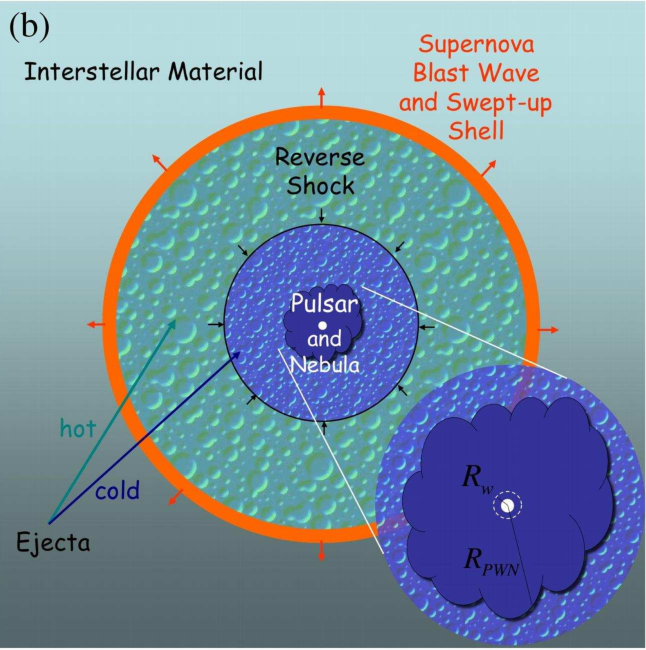
\includegraphics[height=0.4\textwidth]{04_Introduction/Images/pulsar_wind_nebula/pulsar_wind_nebula_structure.pdf}
	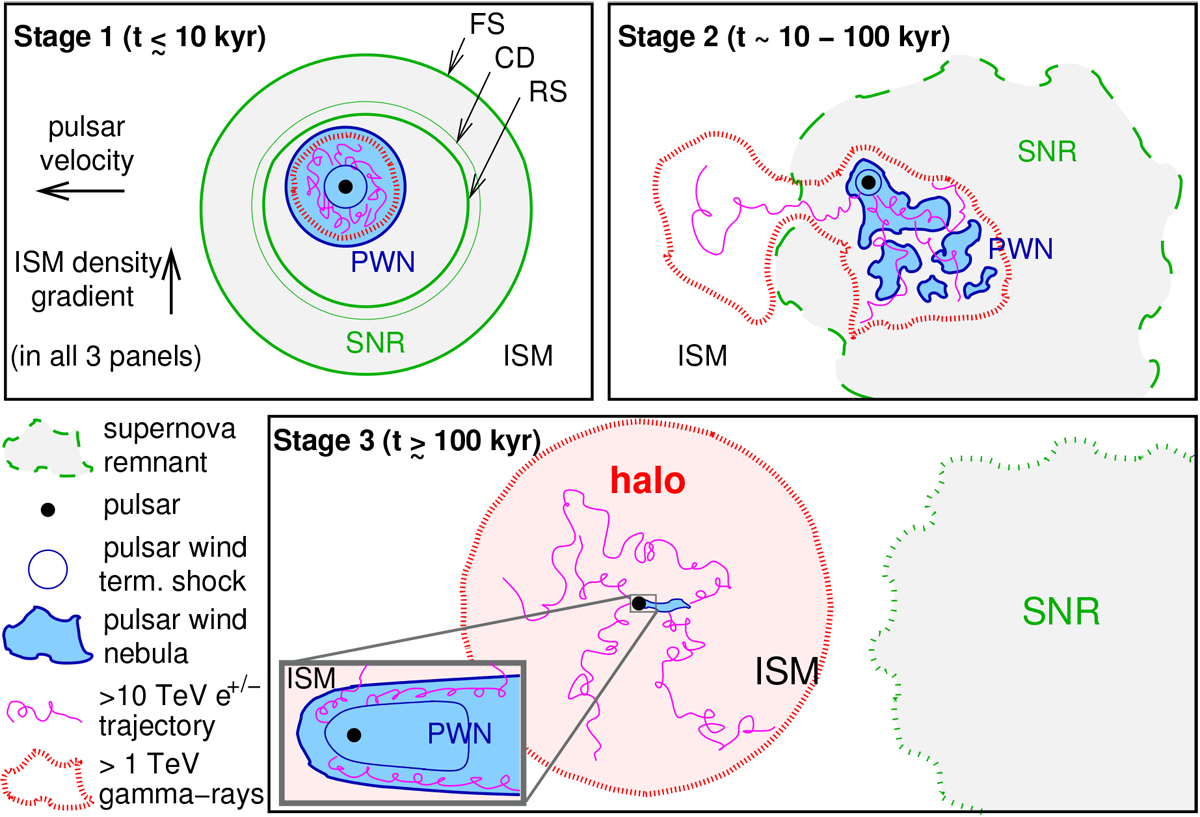
\includegraphics[height=0.4\textwidth]{04_Introduction/Images/pulsar_wind_nebula/pwn_evolution.jpg}
	\caption{(\textit{left}) Structure of a composite SNR and PWN. Image courtesy of \cite{2006ARA&A..44...17G}. (\textit{right}) A PWN evolves within the SNR and is eventually crushed by the reverse shock. The pulsar escapes the SNR and the electrons escaping into the ISM form a TeV halo around the PWN. Image courtesy of \cite{2020A&A...636A.113G}.}
	\label{fig:chapter1_pulsar_wind_nebula_structure}
\end{figure*}

\subsubsection{Stage 1: Expansion Phase ($<10\,\si{\kilo\year}$)}

As the pulsar wind expands into the shocked region of the SNR, the outer winds of the PWN are decelerated by the ISM until the ram pressure of the interstellar wind counteracts the internal pressure of the PWN, $P_\text{PWN}$ (see \autoref{fig:chapter1_pulsar_wind_nebula_structure}). This forms the termination shock at radius \citep{2006ARA&A..44...17G}:

\begin{equation}
    \begin{aligned}
    r_\text{ts}&=\qty(\frac{\dot{E}}{4\pi\omega c P_\text{PWN}})^\half\text{ ,}
    \end{aligned}
\end{equation}
where $\dot{E}$ is the spin-down power and $\omega$ is the filling factor of the PWN ($\omega \approx 1$ for isotropic winds) \citep{2002AstL...28..373B}. Typical PWN have a termination shock occurring at $r_s\approx 0.1\,\pc$ \citep{2006ARA&A..44...17G}. Particles are re-accelerated at the termination shock and are believed to be the source of the radio to unpulsed $\TeV$ emission from PWN. For a PWN in its first stage of evolution, the radius evolves as \citep{10.1007/978-94-010-1229-4_5}:

\begin{equation}
    \begin{aligned}
    r_\text{PWN} &= 1.5\dot{E_0}^\frac{1}{5}E_\text{SNR}^{\frac{3}{10}}M_\text{ej}^{-\frac{1}{2}} t^\frac{6}{5} \text{ ,}
    \end{aligned}
\end{equation}
where $E_\text{SNR}$ and $M_\text{ej}$ are the energy and ejected mass of the SNR respectively. At this stage the spin down energy of the pulsar, $E_0$, is roughly constant.
\newpar 
Asymmetry in the progenitor supernova will result in the pulsar gaining a so-called kick velocity up to $300\,\kmpersec$ \citep{2017ApJ...844....1K}, however at early stages the pulsar appears towards the centre of the SNR. 

\subsubsection{Stage 2: ($10-100\,\kiloyear$)}

As the PWN evolves inside the SNR, the outer edges of the SNR collide with the ISM and forms a reverse shock (see \autoref{appendix:snrs}). The reverse shock travels radially inwards and crushes the PWN, increasing its pressure and magnetic field \citep{2006ARA&A..44...17G}. The pressure inside the PWN increases until it is greater than its surroundings, resulting in a subsonic expansion of the nebula. This compression and expansion phase repeats itself over a time scale of a few thousand years. The crushing of the PWN by the reverse shock is anti-symmetric due to the kick velocity of the pulsar and non-uniformity in the ISM, leading to complex morphology of the PWN.
\newpar 
At the edge of the PWN, $r_\text{PWN}$, the pressure is balanced with that of the associated SNR. During stage 2, the SNR will be in its Sedov-Taylor phase of its evolution (see \autoref{appendix:snrs}) with radius $r_\text{SNR} \propto t^{\frac{2}{5}}$. Therefore, the radius of the PWN is thought to be related to the SNR radius via \citep{2001A&A...380..309V}:

\begin{equation}
    \begin{aligned}
        r_\text{PWN}\propto t^{\frac{1}{3}} r_\text{SNR} \propto t^{11/15}\text{ .}
    \end{aligned}
\end{equation}
\newpar
High-energy electrons can escape the PWN into the ISM and can emit $\TeV$ gamma rays via inverse Compton interactions, forming a $\TeV$ halo \citep{2020A&A...636A.113G}.

\subsubsection{Stage 3: Formation of $\TeV$ halos ($t\gtrsim100\,\kiloyear$)}

At this stage, the kick velocity of the pulsar has allowed it to escape the SNR (which is now fading into the ISM). The pulsar is travelling faster than the speed of sound in the ISM, forming a bow shock with the PWN trailing behind (see \autoref{fig:chapter1_pulsar_wind_nebula_structure}) \citep{2020A&A...636A.113G}. At this point a $\TeV$ halo is formed around the PWN. Extended $\TeV$ emission, indicative of a $\TeV$ halo, has been seen towards the Geminga and \mbox{PSR\,B0656+14} pulsars \citep{2017Sci...358..911A}.

\subsubsection{Time Evolution of the PWN Magnetic Field Structure}

\begin{figure}[h!]
	\centering
    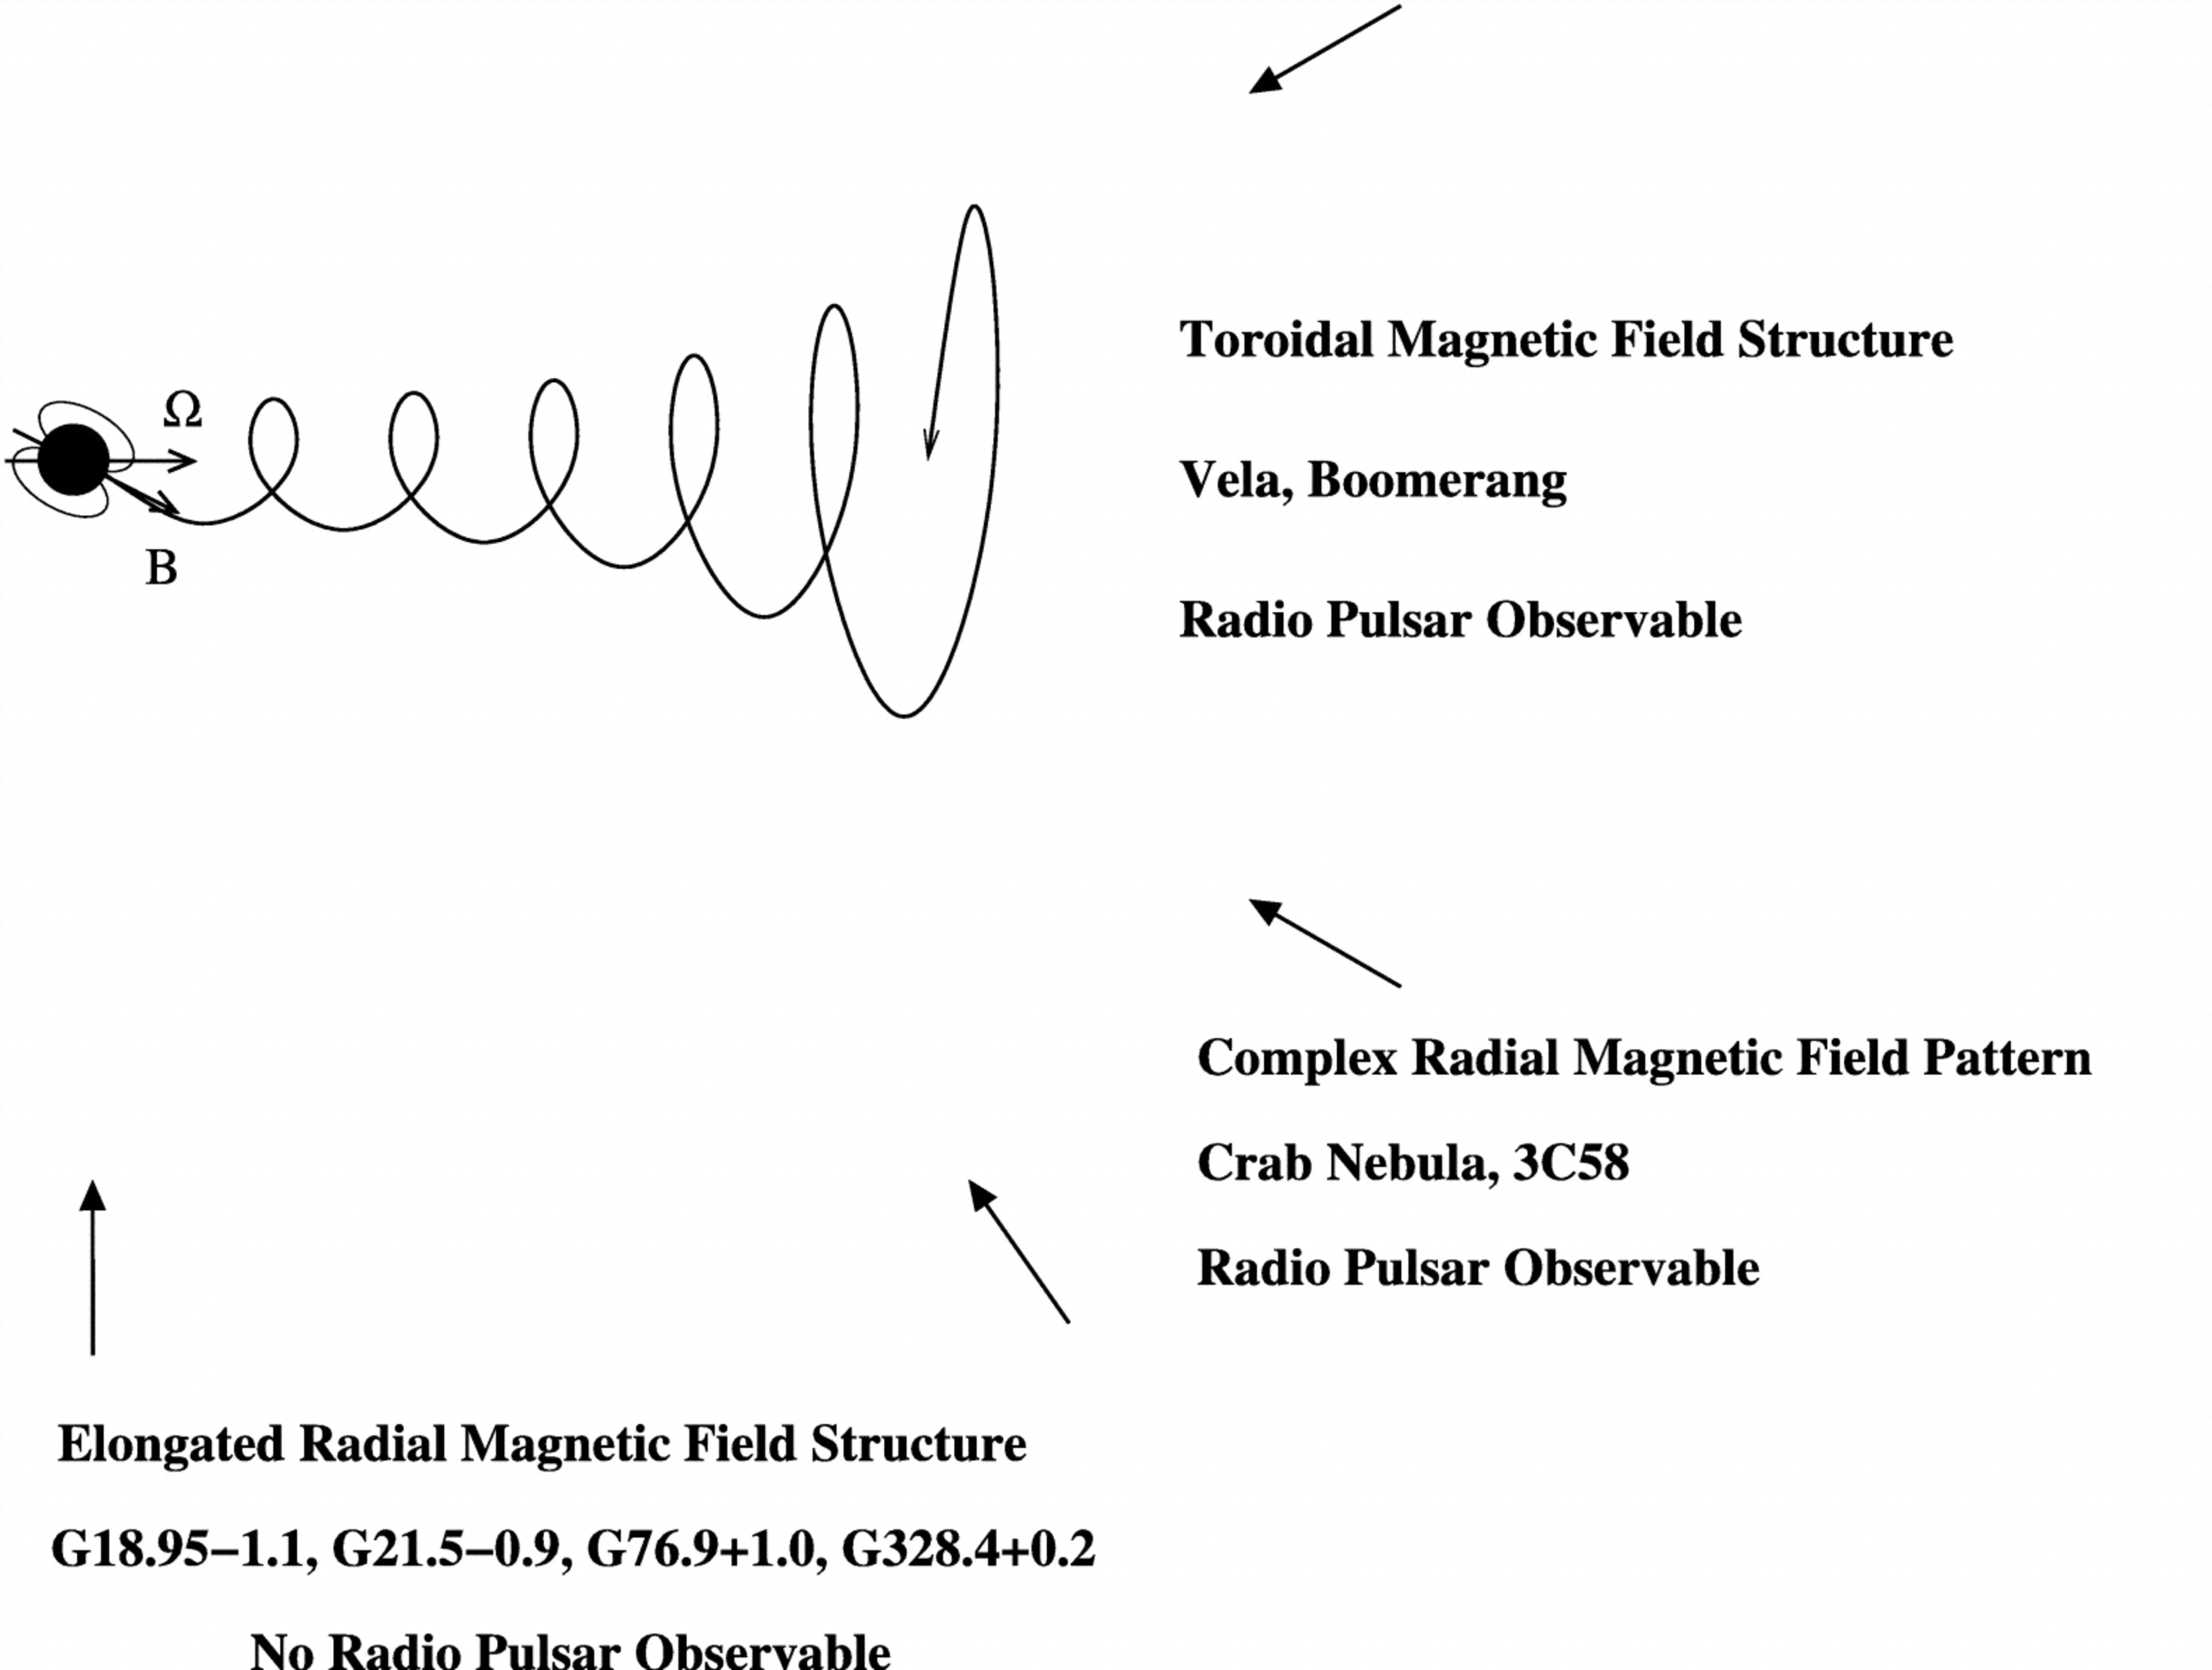
\includegraphics[height=0.22\textheight]{04_Introduction/Images/pulsar_wind_nebula/magnetic_field_structure.pdf}
	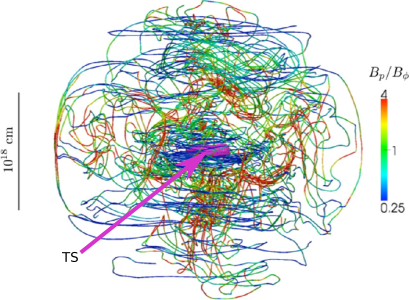
\includegraphics[height=0.22\textheight]{04_Introduction/Images/pulsar_wind_nebula/PWN_magnetic_field_structure.jpeg}
	\caption{(\textit{left}) Expansion of the PWN magnetic field lines and how the viewing angle alters the way the magnetic field structure appears at Earth. Image courtesy of \cite{2006ApJ...638..225K} (\textit{right}) Simulated magnetic field lines of a stage 1 PWN. Azimuthal orientated field lines are shown in blue while radial field lines are shown in red. The termination shock is indicated by magenta and indicated by the arrow. Image adapted from \cite{2014MNRAS.438..278P}}
	\label{fig:chapter1_magnetic_field_structure_PWN}
\end{figure}

The charged winds of PWNe are influenced by the presence of magnetic fields. The magnetic field structure of PWNe is believed to be toroidal in nature, with the viewing angle affecting observations at Earth \citep{2006ApJ...638..225K, 2012SSRv..166..231R}. If the axis of rotation aligns with the viewing angle, the magnetic field appears to be toroidal (see left-hand panel of \autoref{fig:chapter1_magnetic_field_structure_PWN}). In contrast, the magnetic field of the pulsar will appear to be radially dependent if the viewing angle and axis of rotation is perpendicular to each other. More complex observed magnetic field structures occur when the viewing angle is between these two extremes (see the right-hand panel of \autoref{fig:chapter1_magnetic_field_structure_PWN}).
\newpar
The magnetic field evolves with the PWN. The average magnetic field of the PWN, $B_\text{PWN}$, at time $t$ can be found by considering the conservation of magnetic energy density (see \cite{2010ApJ...715.1248T} and references within):

\begin{equation}
    \begin{aligned}
    V_\text{PWN}\frac{B^2_\text{PWN}\qty(t)}{8\pi}&=\int_0^t\eta L\qty(t')\dd{t'} \\
    &=\eta E_\text{spin}\qty(t)\text{ ,}
    \end{aligned} \label{eq:chapter_1_mag  fnetic_conservation_energy}
\end{equation}
\noindent where $V_\text{PWN}$ is the volume of the PWN, $L$ is the injection luminosity of the associated pulsar, $\eta$ ($0\leq\eta\leq 1$) is the ratio of the magnetic energy and the pulsars' spin down power and $E_\text{spin}$ is the time-integrated spin down energy. The resulting magnetic field is then:

\begin{equation}
    \begin{aligned}
    B\qty(t)&=\sqrt{\frac{3\qty(n-1)\eta L_0\tau_0}{R^3_\text{PWN}}\qty[1-\qty(1+\frac{t}{t_0})^{-\frac{2}{n-1}}]}\text{ ,}
    \end{aligned} \label{eq:chapter_1_magnetic_field_ev}
\end{equation}
\noindent where $R_\text{PWN}$ is the size of the PWN and $\tau_0$ is the initial spin down timescale (see \autoref{eq:chapter1_characteristic_age}). For $t>\tau_0$, the magnetic field of the PWN can be approximated by $B\qty(t)\propto t^{-1.5}$.

\subsubsection{Time Evolution of the Spectral Energy Distribution}

\begin{figure}[h!]
    \centering
    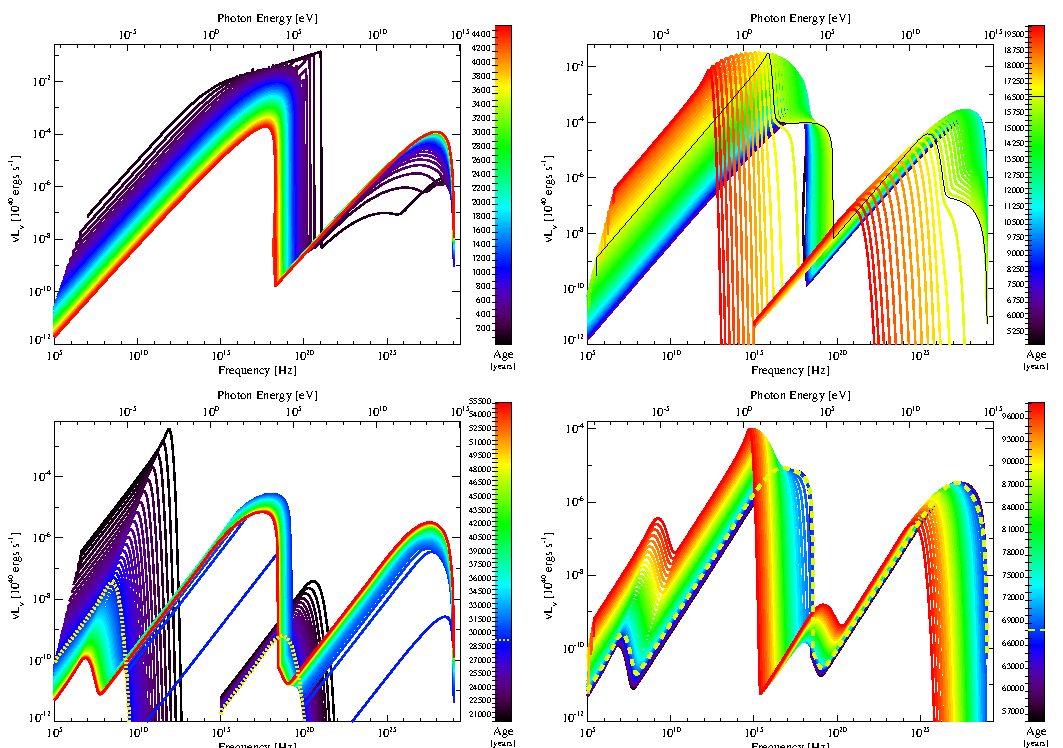
\includegraphics[width=\textwidth]{04_Introduction/Images/pulsar_wind_nebula/pwn_spectra_evolution.pdf}
    \caption{Theoretical time evolution of the multi-wavelength SED of a PWN inside a SNR. See text for more information. Image courtesy of \cite{2009ApJ...703.2051G}.}
    \label{fig:chapter_1_PWN_spectra_evolution}
\end{figure}
A spectral energy distribution (SED) describes how the energy flux of photons (or particles) from a source varies with energy. \autoref{fig:chapter_1_PWN_spectra_evolution} from the study \cite{2009ApJ...703.2051G} shows the SED time evolution for an example PWN with braking index $3$ and electron injection luminosity of $10^{40}\,\ergspersec$, where electrons follow a power-law spectrum ($\propto E^{-1.6}$).
\newpar
At $t=0$ (stage 1), the injected electrons have not experienced any energy losses and form a strong peak in the X-ray regime through synchotron emission. The same electrons will interact with the cosmic microwave background (CMB) through inverse Compton interactions and form a strong peak in the $\GeV$ regime  (top-left panel of \autoref{fig:chapter_1_PWN_spectra_evolution}). As the PWN expands within the SNR, the overall magnetic field strength of the PWN decreases and the synchotron luminosity peak migrates to lower energies in the optical regime. This leaves more energy to be lost through inverse Compton interactions (see \autoref{sec:chapter_1_leptonic_gre}) and the inverse Compton peak transitions from the $\GeV$ to the $\TeV$ regime.
\newpar
As the reverse shock compresses the PWN (stage 2), the increased magnetic field turbulence within the PWN strengthens the magnetic field. Thus, electrons injected into the PWN lose more energy to synchrotron losses and the ratio of synchrotron to inverse Compton flux increases (top-right panel of \autoref{fig:chapter_1_PWN_spectra_evolution}). At this point, two distinct peaks start to form in the synchrotron and inverse Compton spectra due to the two populations of young high-energy electrons and the older lower energy electrons that were initially injected into the PWN. During this compression, the pulsar may leave the PWN due to its kick velocity and no new electrons are injected into the system. The synchrotron and inverse Compton peak from the young high electrons subsequently disappears (black line in the top-right panel of \autoref{fig:chapter_1_PWN_spectra_evolution}).
\newpar
The pressure inside the PWN increases due to compression until it is greater than the surrounding ISM and the PWN expands. Before the pulsar re-enters the PWN, the overall magnetic field strength of the PWN decreases and the inverse Compton flux from the electron population increases at the expense of the synchrotron flux (top-right and bottom-left panel of \autoref{fig:chapter_1_PWN_spectra_evolution}). New electrons are injected in the PWN when the pulsar re-enters the system, creating two populations of old low-energy electrons and young high-energy electrons. This is reflected in the inverse Compton and synchrotron emission (dotted orange line in the bottom-left panel of \autoref{fig:chapter_1_PWN_spectra_evolution}).
\newpar
As the PWN re-expands, the pressure inside the PWN decreases until it less than the pressure due to the associated SNR and the PWN is compressed. Similarly to the first compression, the magnetic field strength inside the PWN increases and the ratio of synchrotron to inverse Compton flux increases. The pulsar will again leave the PWN (dotted yellow line in the bottom right-panel of \autoref{fig:chapter_1_PWN_spectra_evolution}) and no new electrons are injected into the system (stage 3). The synchrotron and inverse Compton peak from the young high-energy electrons migrates to lower energies due to high energy losses. However, the energy of the synchotron peak from old low-energy electrons increases while the energy of the inverse Compton peak decreases as a result of the increasing magnetic field.

\subsection{TeV Pulsar Wind Nebula} \label{sec:01_PWN_TeVPWN}

It was postulated by \cite{1965PhRvL..15..577G} that PWN are a source of $\TeV$ gamma rays via inverse Compton emission. This was confirmed in 1989 when \cite{1989ApJ...342..379W} reported the first detection of $\TeV$ emission from the Crab Nebula. A $\TeV$ PWN is predicted to be physically larger than the X-ray nebula \citep{1997MNRAS.291..162A}.

\begin{figure}[b!]
	\centering
	\begin{subfigure}{0.495\textwidth}
	    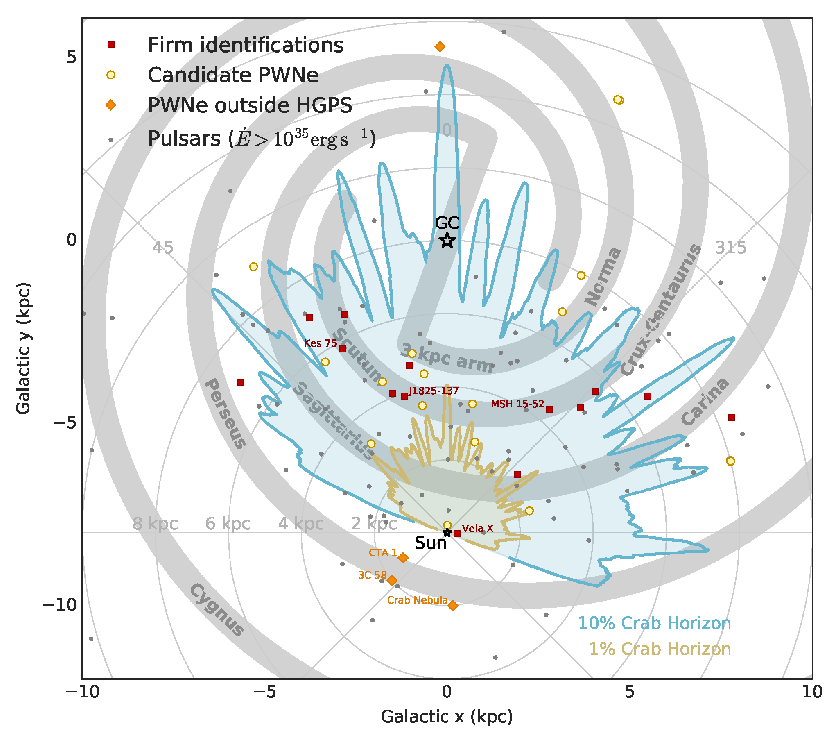
\includegraphics[width=\linewidth]{04_Introduction/Images/pulsar_wind_nebula/TeV_PWN_location.eps}
	\end{subfigure}
	\hfill
	\begin{subfigure}{0.495\textwidth}
	    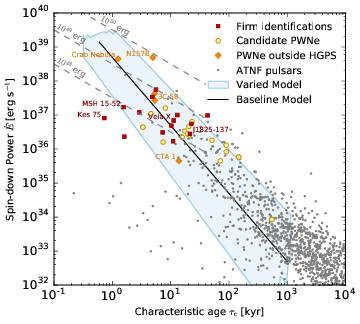
\includegraphics[width=\linewidth]{04_Introduction/Images/pulsar_wind_nebula/pulsar_spin_down_vs_age.png}
	\end{subfigure}
	
	\begin{subfigure}{0.495\textwidth}
	    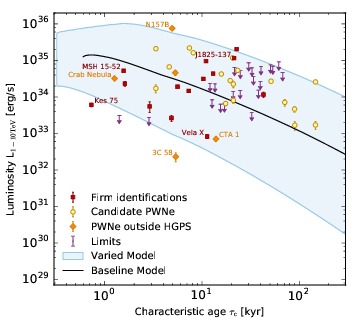
\includegraphics[width=\linewidth]{04_Introduction/Images/pulsar_wind_nebula/pulsar_luminosity_vs_age.png}
	\end{subfigure}
	\hfill
	\begin{subfigure}{0.495\textwidth}
	    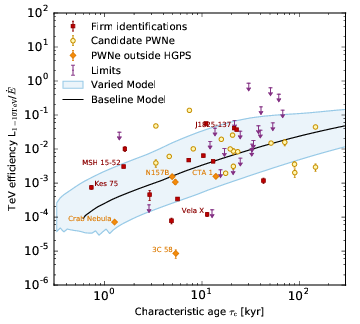
\includegraphics[width=\linewidth]{04_Introduction/Images/pulsar_wind_nebula/pulsar_efficiency_vs_age.png}
	\end{subfigure}
	\caption{(\textit{top-left}) An illustration of the Milky Way spiral arm structure and the location of identified and candidate PWN from the H.E.S.S. HPGS. Spin down power (\textit{top-right}), $\TeV$ luminosity (\textit{bottom-left}) and $\TeV$ efficiency (\textit{bottom-right}) vs the characteristic age of known PWN. Images from  \cite{2018A&A...612A...2H}.}
	\label{fig:chapter1_PWN_properties}
\end{figure}
\newpar
The H.E.S.S. $\TeV$ gamma-ray survey revealed 78 very high-energy (VHE) gamma-ray sources \citep{2018A&A...612A...1H}: 12 are confirmed $\TeV$ PWNe, 8 are composite objects (PWN + SNR) and a further 36 are identified as $\TeV$ PWNe candidates. The H.E.S.S. observatory will be discussed further in \autoref{sec:02_HESS}. \cite{2018A&A...612A...2H} reviewed the H.E.S.S. Galactic Plane Survey (HPGS) in order to investigate the evolution and nature of TeV PWNe. It was found that the majority of PWN are located on or near the Milky Way spiral arms, with the Crux-Scutum arm hosting half of the PWN from the HGPS (see \autoref{fig:chapter1_PWN_properties}).
\newpar
Through time-dependent modelling of $\TeV$ PWN \citep{2018A&A...612A...2H} it was noted that as PWNe age:

\begin{enumerate}
    \itemsep0em
    \item The physical offset between the pulsar and TeV PWN increases (at a rate of $\approx 0.5\si{pc\per\kilo\year}$) due to the kick-velocity of the pulsar and the SNR reverse shock crushing the PWN.
    \item The TeV luminosity ($L_{1-10\,\TeV}$) of known PWN varies widely with characteristic age (from $\approx 10^{35}\,\ergspersec$ at $1\,\kiloyear$ to $\approx 10^{34}\,\ergspersec$ at $10\,\kiloyear$) with no clear statistical correlation.
    \item The TeV efficiency ($L_{1-10\,\TeV}/\dot{E}$) increases (from $2\times 10^{-4}$ at $1\,\kiloyear$ to $3\times 10^{-3}$ at $10\,\kiloyear$) possible due to the physical offset between the pulsar and TeV PWN.
\end{enumerate}

\subsection{Mysteries of Pulsar Wind Nebulae} \label{sec:chapter_1_mystery_PWN}

Even though multiple PWNe have been observed and studies such as \cite{2018A&A...612A...2H} have modelled trends of $\TeV$ PWN, there are still many open questions. The following will summarise some of these questions.

\subsubsection{How are electrons transported within pulsar wind nebula?}

Electrons released by a pulsar are subject to varying transport processes and energy losses. In a non-uniform environment (due to gas and magnetic field turbulence), electrons scatter off the ISM atoms and magnetic field turbulence resulting in diffusive motion outwards from the acceleration site (see \autoref{chapter_1_cr_propagation}). Electrons in PWNe may also experience an overlying bulk transport in a particular direction, i.e. advection. It has been proposed that advection dominates the particle transport close to the pulsar while diffusion dominates the outer reaches of the nebula \citep{2020A&A...636A.113G, 2021PhRvD.104l3017R}. Electrons undergo energy losses through inverse Compton, synchrotron and Bremsstrahlung emission (see section \autoref{sec:chapter_1_leptonic_gre}). The rate at which an electron loses energy depends heavily on the surrounding environment.
\newpar
A challenge in modelling PWN will be balancing the transport of electrons and energy losses with respect to the surrounding environment in order to explain the multi-wavelength emission.

\subsubsection{Can pulsar wind nebula accelerate particles up to $\PeV$ energies?}

The steepening of the cosmic-ray proton and nuclei spectrum at earth between the knee ($1\,\PeV=10^{15}\,\eV$) and the ankle ($10^{18}\,\si{\exa\electronvolt}$) from $E^{-2.7}$ to $E^{-3}$ suggests the transition from Galactic to extra-Galactic cosmic rays occurs between (see \autoref{sec:chapter_1_cr_spectrum}). Additionaly, the confinement time of cosmic rays within the galaxy suggests that sources must provide $10^{41}\,\ergspersec$ to explain the observed cosmic ray intensity. Thus, what type of Galactic source is capable of accelerating cosmic rays up to PeV energies, i.e. a PeVatron (see \autoref{sec:chapter_1_PeVatrons})?
\newpar
Due to their large energy budget ($\approx 10^{51}\,\ergs$ of kinetic energy) and production rate ($\approx 2-3$ supernova occur in the Milky Way per century), SNRs have been the most likely candidates for Galactic PeVatrons \citep{1983A&A...125..249L, 1984ARA&A..22..425H,2004MNRAS.353..550B,10.1093/mnras/sty1589}. Recently, the suitability of SNRs by themselves as PeVatrons has been called into question \citep{CRISTOFARI2020102492} and PWNe are now being considered as additional candidates \citep{2018MNRAS.478..926O, Xin_2019, de_O_a_Wilhelmi_2022,2022A&A...660A...8B}.
\newpar
In 2021, the LHAASO facility identified 12 gamma-ray sources with the detection of photons between $100\,\TeV$ to $1.4\,\PeV$ \citep{2021Natur.594...33C}. These sources are prime PeVatron candidates; two being firmly identified PWNe and a further nine having possible PWN counterparts. One of the twelve PeVatron candidates is the Crab Nebula. The $\MeV$ synchrotron emission from the Crab Nebula and maximum gamma-ray energy of $\approx 0.9\,\PeV$ heavily implies the presence of $\PeV$ electrons within the nebula \citep{doi:10.1126/science.abg5137}.

\subsubsection{Is there a hadronic component to the pulsar wind nebula?}

Spectral and spatial analysis of known PWNe indicate that leptonic emission is the main source of gamma-ray emission. With the detection of $\PeV$ emission towards known PWNe \citep{doi:10.1126/science.abg5137}, further studies suggest that PWN may have an additional hadronic component \citep{2006A&A...451L..51H, 10.1111/j.1745-3933.2010.00934.x, Xin_2019, 2021ApJ...922..221L}. The majority of literature consider the winds of the PWN to consist of electrons and positrons (e.g. \cite{2018A&A...612A...2H}). However, in the polar cap model (see \autoref{fig:chapter1_magnetosphere_structure}) electrons, positrons and protons are stripped from the surface of the pulsar. \cite{1994ApJ...435..230G} proposed that a fraction of the spin-down power of the pulsar is converted into a wind of protons. These protons undergo proton-proton collisions to produce pions (see \autoref{sec:chapter1_hadronic_gr_emission}). Charged pions decay into muons, which subsequently decay into electrons and positrons. \cite{2003A&A...402..827A} suggested that signatures of these `secondary' electrons/positrons can be found in the production of $\TeV$ gamma rays and neutrinos. Moreover, the SNR reverse shock can re-introduce protons into the PWN and accelerate protons to greater than $1\,\PeV$ \citep{1992MNRAS.257..493B,2018MNRAS.478..926O}. The observation of neutrino emission from PWN through the decay of charged muons acts as a signature of hadronic gamma-ray production \citep{2006A&A...451L..51H}. However, leptonic-hadronic modelling towards the Crab PWN suggests that the resulting neutrino flux would be below the sensitivities of current neutrino observatories \citep{2022ApJ...926....7P}.

\subsection{HESS J1825-137 and HESS J1826-130} \label{sec:01_1825_1826}

% 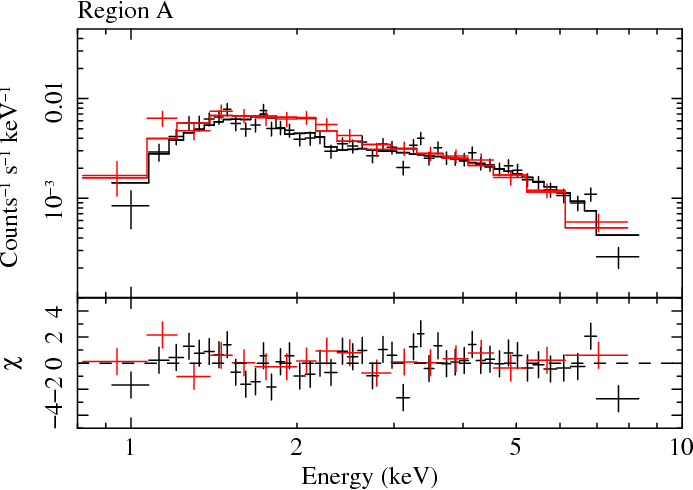
\includegraphics[width=0.5\textwidth]{04_Introduction/Images/pulsar_wind_nebula/1825_xray_flux.png}

This thesis will focus on the PWN associated with $\TeV$ source \mbox{HESS\,J1825-137}. The following will briefly summarise the literature of \mbox{HESS\,J1825-137} and nearby $\TeV$ source \mbox{HESS\,J1826-130}.
\newpar
\begin{figure}[h!]
	\centering
	% 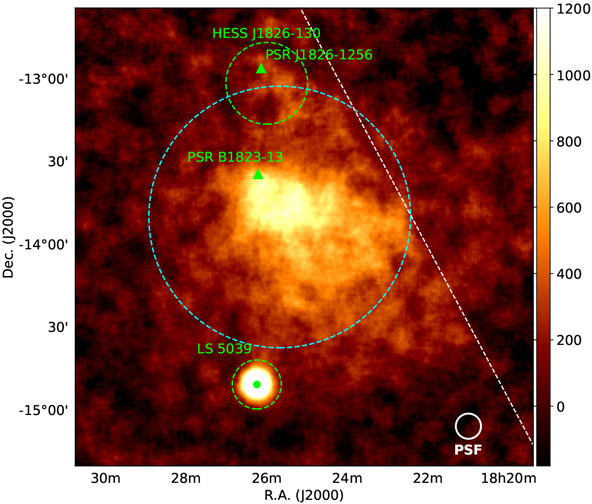
\includegraphics[height=0.23\textheight]{04_Introduction/Images/pulsar_wind_nebula/1825_morphology.jpg}
	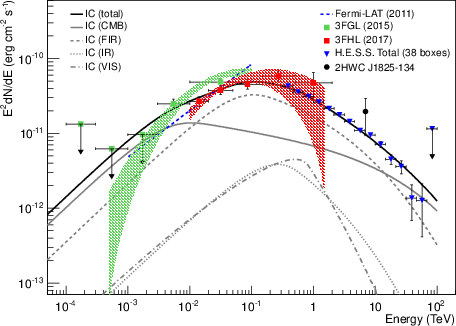
\includegraphics[height=0.2\textheight]{04_Introduction/Images/pulsar_wind_nebula/1825_energy_flux.png}
    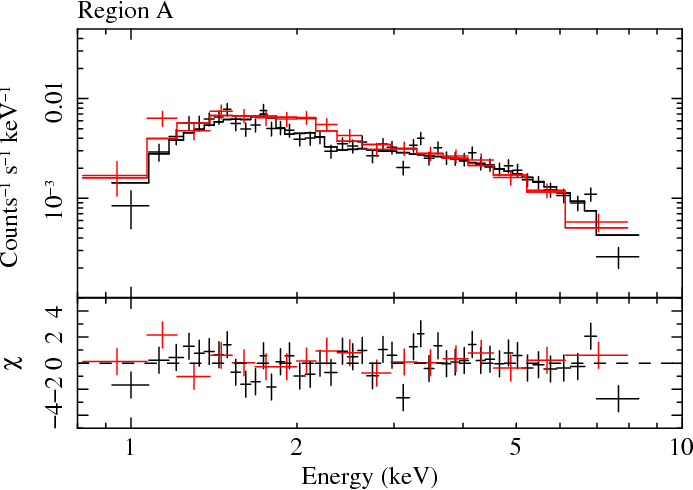
\includegraphics[height=0.2\textheight]{04_Introduction/Images/pulsar_wind_nebula/1825_xray_flux.png}
    \caption{(\textit{left}) Gamma-ray SED of \mbox{HESS\,J1825-137} as seen by HESS together with the \textit{Fermi}-LAT 3FGL and 4FHL equivalent sources. (\textit{right}) X-ray SED towards \mbox{PSR\,J1826-1334}. Images courtesy of \cite{2019A&A...621A.116H} and \cite{2009PASJ...61S.189U}.}
    \label{fig:chapter1_hess_j1825_morphology_paramaters}
\end{figure}
\begin{SCfigure}[0.67][h!]
    \centering
    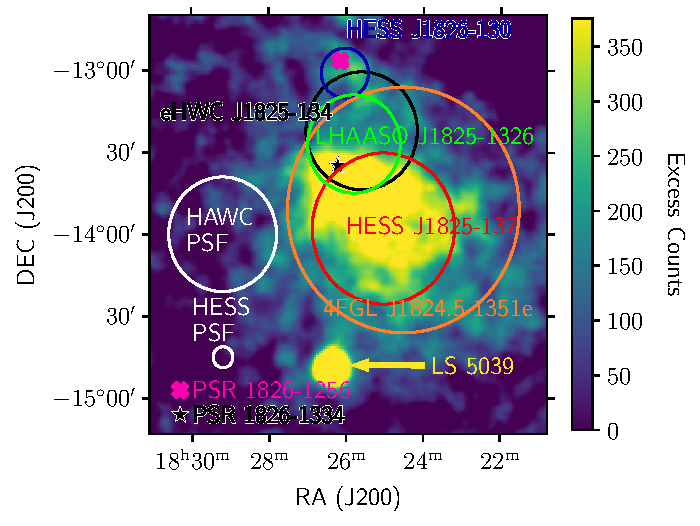
\includegraphics[width=0.6\textwidth]{04_Introduction/Images/pulsar_wind_nebula/hess_j1825_image.pdf}
    \caption{HESS excess counts map towards \mbox{HESS\,J1825-137} from \cite{2019A&A...621A.116H}. The spatial position and extent of \mbox{HESS\,J1825-137} and the equivalent \textit{Fermi}-LAT, HAWC and LHAASO sources are shown together with PSR\,J1826-1334 (star) and PSR\,J1826-1256 (cross).}
    \label{fig:chapter1_hess_j1825_137_object_positions}
\end{SCfigure}


\begin{table}[h!]
    \caption{Fit parameters to the spectrum of \mbox{HESS\,J1825-137} and equivalent \textit{Fermi}-Lat and HAWC sources. Power law (PL): $\dv{N}{E}\propto \qty(\frac{E_p}{E_0})^{-\Gamma}$. Exponential Cutoff Power Law (ECPL): $\dv{N}{E}\propto \qty(\frac{E_p}{E_0})^{-\Gamma}\exp(-\frac{E}{E_c})$. Log Parabola (LP): $\dv{N}{E}\propto \qty(\frac{E_p}{E_0})^{-\qty[\Gamma+\beta\log(E/E_0)]}$. Broken Power Law (BPL: $\dv{N}{E}\propto \qty(\frac{E_p}{E_b})^{-\Gamma}$ where $\Gamma=\Gamma_1$ if $E<E_b$ and $\Gamma=\Gamma_2$ otherwise. $E_0=1\,\TeV$ unless specified.}
    \resizebox{\textwidth}{!}{
    \begin{threeparttable}
    \centering
    \begin{tabular}{rllllll}
        \toprule
        Model & $\Gamma$ & Parameters & RA & DEC & extent ($^\circ$) & References \\
        \midrule 
        \textbf{HESS J1825-137} & - & - & $18\si{\hour}25\si{m}49\si{\second}$ & $-\ang{13}46\si{m}35\si{\second}$ & $0.66^*$ & a \\
        PL & $2.23\pm0.02\pm0.04$ & - & - & - & - & a \\
        ECPL & $2.06\pm0.05\pm0.08$ & $E_c = 15\pm5\pm6\,\TeV$ & - & - & - & a \\
        LP &  $2.21\pm0.03\pm0.04$ & $\beta=0.08\pm 0.02\pm 0.03$ & - & - & - & a \\
        \textbf{4FGL\,J1824.5-1351e} & - & - & $18\si{\hour}24\si{m}31.2\si{\second}$  & $-\ang{13}51\si{m}07.2\si{\second}$  & $0.75$ & b \\
        LP & $1.96\pm0.68$ & $E_0 = 145\pm\,\GeV$ & - & - & - & c \\
        & - & $\beta$ = $0.046\pm 0.013$ & - & - & - & - \\
        BPL & $1.70\pm0.04$ & $E_b = 115\pm8\,\GeV$ & - & - & - & c \\
        & $2.29\pm0.15$ & - & - & - & - & - \\
        \textbf{3HWC J1825 - 134} & - & - &  $18\si{\hour}25\si{m}50.4\si{\second}$ & $-\ang{13}24\si{m}03.6\si{\second}$ & - & d  \\
        PL & $2.35\pm0.02$ & - & - & - & - & d \\
        \textbf{eHWC J1825 - 134} & - & - &  $18\si{\hour}25\si{m}36\si{\second}$ & $-\ang{13}22\si{m}12\si{\second}$ & $0.34$ & e  \\
        ECPL  & $2.12\pm0.15$ & $E_c = 61\pm12\,\TeV$  & - & - & - & e \\
        \textbf{LHAASO\,1825-1326} & - & - & $18\si{\hour}25\si{m}48\si{\second}$ & $-\ang{13}27\si{m}00\si{\second}$ & $0.3$ & f \\
        \bottomrule
    \end{tabular}
    \begin{tablenotes}
	\item $^*$: Average of the southern and northern extent 
	\item \textbf{References}
	\item a: \citep{2019A&A...621A.116H}
	\item b: \citep{2020ApJS..247...33A}
	\item c: \citep{2020A&A...640A..76P}
	\item d: \citep{2020ApJ...905...76A}
	\item e: \citep{PhysRevLett.124.021102}
    \item f: \citep{2021Natur.594...33C}
    \end{tablenotes}
    \end{threeparttable}
    }
    \label{tab:chapter1_1825_parameters}
\end{table}
Discovered in $2005$, \mbox{HESS\,J1825-137} is one of the most luminous and extensive $\TeV$ PWN \citep{2005A&A...442L..25A,2006A&A...460..365A}. \mbox{HESS\,J1825-137} is powered by \mbox{PSR\,J1826-1334}, which has a spin down power, period, period derivative and DM distance of $2.8\times 10^{36}\,\ergspersec$, $101.5\,\si{\milli\second}$, $7.5\times 10^{-14}\,\si{\second\per\second}$ and $3.6\,\kpc$ respectively \citep{2005AJ....129.1993M}. \autoref{eq:chapter1_characteristic_age} gives the characteristic age of PSR\,J1826-1334 as $21.4\,\si{\kiloyear}$, placing the PWN in its second phase of its evolution (see \autoref{sec:01_intro_time_ev_PWN}). In support of this, a $\TeV$ halo appears to be forming around \mbox{HESS\,J1825-137} \citep{2020A&A...640A..76P}. The High Altitude Water Cherenkov (HAWC) observatory has observed gamma rays towards equivalent source \mbox{eHWC\,J1825-134} with energies greater than $100\,\TeV$ \citep{PhysRevLett.124.021102}. Similarly, LHAASO identified \mbox{HESS\,J1825-137} (LHAASO\,J1825-1326) as a possible PeVatron candidate (see section.\,\autoref{sec:chapter_1_PeVatrons}) \citep{2021Natur.594...33C}. The equivalent $\GeV$ \textit{Fermi}-LAT source is \mbox{4FGL\,J1824.5-1351e}.  See \autoref{tab:chapter1_1825_parameters} and \autoref{fig:chapter1_hess_j1825_137_object_positions} for the spectral and spatial information of \mbox{HESS\,J1825-137} and equivalent sources.
\newpar
The $\TeV$ morphology towards \mbox{HESS\,J1825-137} (see \autoref{fig:chapter1_hess_j1825_137_object_positions}) is asymmetric around the pulsar, with more extensive emission towards the southern side of the nebula (in Galactic coordinates). The extent (defined to be the point at which the emission drops to $1/e$ of its highest value) towards the south of \mbox{HESS\,J1825-137} was found to be $\ang{0.66}\pm\ang{0.03}_\text{stat}\pm\ang{0.04}_\text{sys}$, while the northern side is extended by $\ang{0.41}\pm\ang{0.03}_\text{stat}\pm\ang{0.09}_\text{sys}$ \citep{2019A&A...621A.116H} . At a distance of $4.0\,\kpc$, this equates to a physical distance of $91\pm4\pm6\,\pc$ and $57\pm4\pm13\,\pc$ to the south and north respectively. The southern side of the nebula is also extensive in $\GeV$ gamma rays as revealed by \cite{2019MNRAS.485.1001A}. This region of gamma-ray emission has a hard spectrum with a photon index of $1.9$ and is suggested to be powered by high-energy electrons from the PWN associated with \mbox{HESS\,J1825-137}.
\newpar
The progenitor SNR associated with \mbox{HESS\,J1825-137} will likely be in its Sedov-Taylor phase of evolution based on the characteristic age of \mbox{PSR\,J1826-1334} (see \autoref{appendix:snrs}). \cite{2001A&A...380..309V} suggests that the size of a SNR will be approximately four times the size of the PWN. The radius of the $\TeV$ PWN associated with \mbox{HESS\,J1825-137} is $38\,\pc$ for a distance of $4\,\kpc$ (see \autoref{tab:chapter1_1825_parameters}), giving an estimated SNR radius of $150\,\pc$. \cite{2016MNRAS.458.2813V} noted a large H$\alpha$ rim-like structure indicative of a SNR shock lying $120\,\pc$ to the south of \mbox{PSR\,J1826-1334}, which is consistent with the predicted SNR size. \cite{2016MNRAS.458.2813V} further postulated a connection between this H$\alpha$ rim and a second H$\alpha$ rim (discovered by \cite{2008MNRAS.390.1037S}) lying at a similar angular distance to the pulsar.

\subsubsection{HESS\,J1826-130}
\begin{figure}[b!]
	\centering
	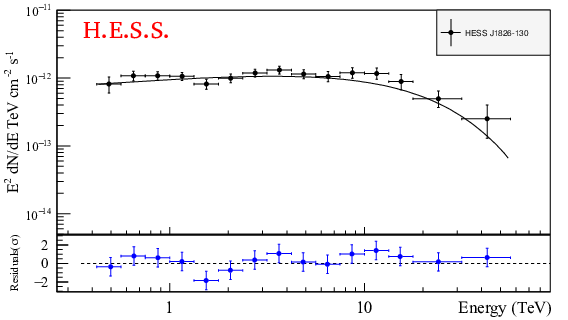
\includegraphics[height=0.18\textheight]{04_Introduction/Images/pulsar_wind_nebula/1826_energy_flux.png}
    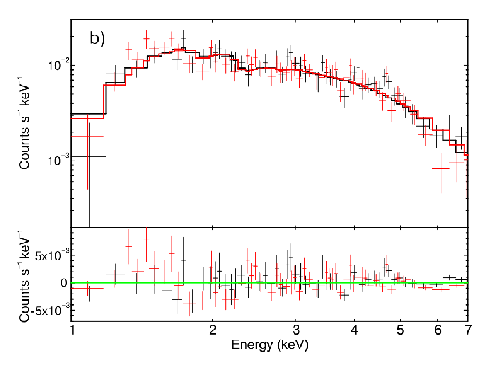
\includegraphics[height=0.18\textheight]{04_Introduction/Images/pulsar_wind_nebula/hess_j1826_130_xray.eps}
	\caption{$\TeV$ (\textit{left}) and X-ray (\textit{right}) SED towards \mbox{HESS\,J1826-130} as seen by H.E.S.S. and Suzaku respectively. Images courtesy of \cite{2020A&A...644A.112H} and \cite{2019A&A...623A.115D} respectively.}
	\label{fig:chapter1_hess_j1826_SED}
\end{figure}


\begin{table}[h!]
    \caption{Fit parameters to the spectrum of \mbox{HESS\,J1826-130}. Power law (PL): $\dv{N}{E}\propto \qty(\frac{E_p}{E_0})^{-\Gamma}$. Exponential Cutoff Power Law (ECPL): $\dv{N}{E}\propto \qty(\frac{E_p}{E_0})^{-\Gamma}\exp(-\frac{E}{E_c})$. Broken Power Law (BPL): $\dv{N}{E}\propto \qty(\frac{E_p}{E_b})^{-\Gamma}$ where $\Gamma=\Gamma_1$ if $E<E_b$ and $\Gamma=\Gamma_2$ otherwise. $E_0=1\,\TeV$ unless specified.}
    \resizebox{\textwidth}{!}{
    \begin{threeparttable}
    \centering
    \begin{tabular}{rllllll}
        \toprule
        Model & $\Gamma$ & Parameters & RA & DEC & extent ($^\circ$) & References \\
        \midrule
        \textbf{HESS J1826-130} & - & - & $18\si{\hour}26\si{m}02.1\si{\second}$ & $-\ang{13}01\si{m}02.6\si{\second}$ & $0.15^*$ & a \\
        PL & $2.12\pm0.04$ & - & - & - & - & a \\
        ECPL & $1.78\pm0.10$ & $E_c = 15.2\pm5$ & - & - & - & a \\
        BPL & $1.96\pm0.06$ & $E_b = 11.2\pm2.7\,\TeV$ & - & - & - & a \\
        & $3.59\pm0.69$ & - & - & - & - & - \\
        \bottomrule
    \end{tabular}
    \begin{tablenotes}
	\item \textbf{References}
	\item a: \citep{2020A&A...644A.112H}
    \end{tablenotes}
    \end{threeparttable}
    }
    \label{tab:chapter1_1826_parameters}
\end{table}

\begin{figure}[ht]
    \centering
    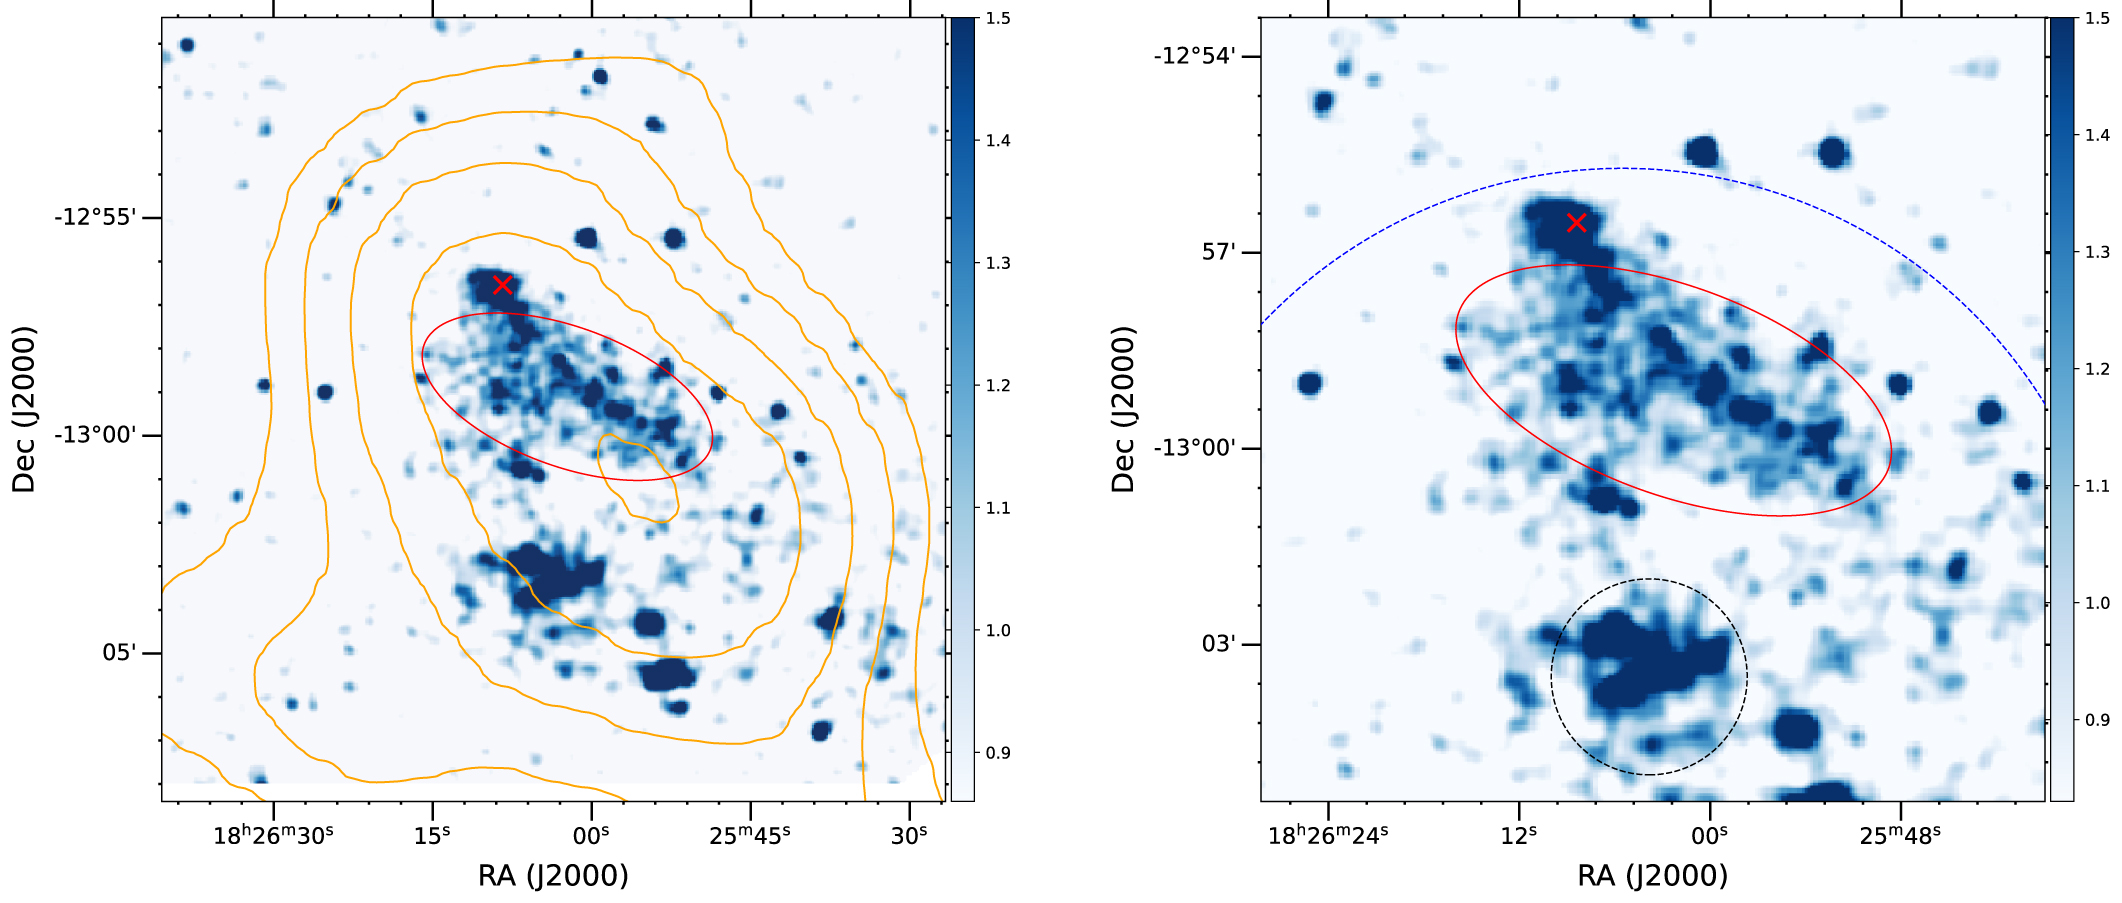
\includegraphics[width=0.9\textwidth]{04_Introduction/Images/pulsar_wind_nebula/hess_j1826_130_xray.jpg}
    \caption{XMN-Newton $0.5-10\,\keV$ X-ray images towards \mbox{HESS\,J1826-130}. The positions of \mbox{PSR\,1826-1256} and the Eel Nebula are shown by the red cross and ellipse respectively. The orange lines represent the H.E.S.S. $3\sigma$ and $5\sigma$ significance contours. Nearby \mbox{SNR\,G18.45-0.42} and star cluster \mbox{Bica 3} are shown by the dashed blue and black circles respectively.  Image courtesy of \cite{2022ApJ...930..148B}.}
    \label{fig:chapter1_hess_j1826_xray}
\end{figure}

\mbox{HESS\,J1826-130} is an unidentified gamma-ray source situated $\approx\ang{0.7}$ to the Galactic north of \mbox{HESS\,J1825-137} (see \autoref{fig:chapter1_hess_j1825_137_object_positions}). Due to its proximity, \mbox{HESS\,J1826-130} was originally thought to be an extension of \mbox{HESS\,J1825-137} until it was classified as a separate source through its energy-dependent morphology \citep{2017AIPC.1792d0024A}. \mbox{HESS\,J1826-130} becomes more distinct from \mbox{HESS\,J1825-137} at higher gamma-ray energies. The analysis conducted by \cite{2020A&A...644A.112H} showed that \mbox{HESS\,J1825-137} contaminates the SED of \mbox{\mbox{HESS\,J1826-130}} by approximately $40\%$ below $1.5\,\TeV$ and $20\%$ above $1.5\,\TeV$. As shown by \autoref{fig:chapter1_hess_j1825_137_object_positions}, the position of \mbox{eHWC\,J1825-134} lies approximately midway between \mbox{HESS\,J1825-137} and \mbox{HESS\,J1826-130}. Due to the coarse angular resolution of HAWC, \mbox{eHWC\,J1825-134} may represent the combined emission from both \mbox{HESS\,J1825-137} and \mbox{HESS\,J1826-130}.
\newpar
Several objects towards \mbox{HESS\,J1826-130} have been associated with the gamma-ray emission based on spatial correlation. This includes the Eel nebula (\mbox{PWN\,G18.5-0.4}), a PWN with a long faint trail ($\ang{0.1}$) of hard X-ray emission above $2\,\keV$ (see \autoref{fig:chapter1_hess_j1826_xray}) \citep{2007whsn.conf...24R,2022ApJ...930..148B}.  Similarly, \cite{2018A&A...612A...1H} proposed two possible SNRs as a source of protons interacting with the interstellar gas to produce the observed gamma-ray emission; \mbox{SNR\,G018.1-0.1} and \mbox{SNR\,G018.6-0.2.} As shown by the purple cross in \autoref{fig:chapter1_hess_j1825_137_object_positions}, \mbox{PSR\,1826-1256} is located towards \mbox{HESS\,J1826-130} and may be a source of electrons powering the PWN. \mbox{PSR\,1826-1256} has spin down power and characteristic age of $3.6\times10^{36}\,\ergspersec$ and $14\,\kiloyear$ respectively \citep{2010ApJS..187..460A}. %The lack of DM distance measurements to the pulsar makes it difficult to solidify its connection to the Eel nebula, \mbox{HESS\,J1826-130} and the aforementioned SNRs.
\newpar
\cite{2016MNRAS.458.2813V} revealed dense turbulent molecular gas between \mbox{HESS\,J1825-137} and \mbox{HESS\,J1826-130}. The same study places the majority of these clouds in the $40-60\,\kmpersec$ velocity range, equivalent to a distance of $3.5-4.5\,\kpc$ as given by the Galactic rotation model (see \autoref{sec:06_galactic_rotation} \citep{1993A&A...275...67B}). This is consistent with the DM distance of \mbox{PSR\,J1826-1334}. Therefore, protons from the associated SNR may interact with these dense clouds through p-p collisions (see \autoref{sec:chapter1_hadronic_gr_emission}) to emit the high-energy gamma rays as seen by \mbox{eHWC\,J1825-134}.

\section{Cosmic Rays} \label{sec:01_cosmic_rays}

As discussed in \autoref{sec:01_PWN}, PWN are a source of high-energy cosmic rays. Therefore, it is vital to understand the properties of cosmic rays in order to explain PWN characteristics.
\begin{figure}[b!]
	\centering
	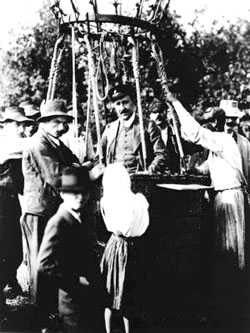
\includegraphics[width=0.7\textwidth]{04_Introduction/Images/History/hess_balloon_flight.jpg}
	\caption{Victor HESS about to ascend to an altitude $>5\,\si{\kilo\meter}$ to discover cosmic rays \citep{hess1912observations}}
	\label{fig:chapter1_hess_balloon_flight}
\end{figure}
\newpar 
In 1896 Henri Becquerel discovered that uranium salts emitted a form of invisible radiation that could penetrate through solid matter. At the beginning of the 20th century, it was generally believed that only elements in the Earth could emit such radiation. However, in 1912, Victor HESS ascended $5\,\km$ with an electroscope in a hot air balloon. He noticed that as altitude increased, the amount of radiation measured by the electroscope increased \citep{hess1912observations}. In contrast, Millikan submerged electroscopes in Muir Lake located in the Rocky Mountains \citep{1926PhRv...28..851M}.  As the electroscopes descended, less radiation was detected. The findings of Hess and Millikan showed that ionising radiation, later dubbed `cosmic rays', originate from the sky. In the mid 20th century, the level of cosmic-ray ionisation was found to be dependent on latitude due to deflection by the Earth's magnetic field \citep{1960Natur.187.1099S}.
\newpar
Cosmic rays comprise of protons, electrons, nuclei, neutrinos and anti-matter. Within this thesis, cosmic rays will be referred to as protons and electrons. Protons consist of three quarks (two up and one down-quark) and are classified as hadrons, a composite subatomic particle made of two or more quarks held together by the strong force. Meanwhile, electrons are elementary particles that belong in the lepton `family' in the standard model of particle physics. Hence, hadronic cosmic rays refer to protons while leptonic cosmic rays refer to electrons.
\newpar 
Supernovae were proposed as a source for cosmic rays by \cite{1934PNAS...20..259B} in the 1930s. In his 1949 paper, Enrico Fermi provided a method where cosmic rays are accelerated by magnetic field irregularities in ISM gas clouds. Fermi's original theory was then modified to consider the acceleration of cosmic rays as they travel through a shock wave generated by, for example, SNRs \citep{1977DoSSR.234.1306K,1977ICRC...11..132A,1978MNRAS.182..147B,1978MNRAS.182..443B,1978ApJ...221L..29B}. SNRs also accelerate cosmic-ray electrons up to high energies as indicated by X-ray emission from synchrotron radiation at the rims of SNRS such as \mbox{SN\,1006} \citep{1995Natur.378..255K}.
\newpar
Other sources that have been proposed as accelerators of cosmic rays include PWN (as discussed in \autoref{sec:01_PWN}), star clusters, binary systems and active Galactic nuclei.

\subsection{Acceleration of Charged Particles}

\subsubsection{Acceleration by pulsars}

As discussed in \autoref{sec:01_PWN_pulsar}, pulsars are the highly dense, magnetised remnants of a supernova. The Lorentz equation,

\begin{equation}
    \begin{aligned}
        \vec{F}=q\vec{E} + q\vec{v}\times \vec{B}\text{ ,}
    \end{aligned} \label{eq:chapter_1_lorentz_force}
\end{equation}

\noindent shows that a magnetic field of strength $\vec{B}$ applies a perpendicular force, $\vec{F}$, on a particle with charge $q$ and velocity $\vec{v}$. In other words, a uniform magnetic field does not change the energy of the particle. However, the rotation of a pulsar coupled with its strong magnetic field generates an electric field, $\vec{E}$. This is described by Faraday's law:
 
 \begin{equation}
    \begin{aligned}
    \nabla \times \vec{E} &= -\pdv{\vec{B}}{t}\text{ .}
    \end{aligned} \label{eq:chapter_1_maxwell_faraday_law_p1}
\end{equation}

\noindent The integral form of \autoref{eq:chapter_1_maxwell_faraday_law_p1} describes a changing magnetic field across a surface with cross sectional area  $\dd{\vec{A}}$:

\begin{equation}
    \begin{aligned}
    \oint_S \vec{E}\cdot \dd{\vec{l}}&=-\int_S \pdv{\vec{B}}{t} \cdot \dd{\vec{A}}\text{ .}
    \end{aligned} \label{eq:01_intro_alven_eq}
\end{equation}

\noindent Where the cross sectional area is the area swept up by expanding surface $S$ in segment $\dd{\vec{\ell}}$ with velocity $\vec{v}_p$ over time $\dd{t}$ ($\dd{\vec{A}}=\dd{\vec{\ell}}\times \vec{v}\dd{t}$). \autoref{eq:01_intro_alven_eq} becomes: 

\begin{equation}
    \begin{aligned}
    \oint_S \vec{E}\cdot \dd{\vec{l}}&=-\int_S \vec{v}_p\times \vec{B}\cdot \dd{\vec{\ell}}\text{ .}
    \end{aligned} \label{eq:chapter_1_maxwell_faraday_law_p2}
\end{equation}

\noindent i.e. the electric field generated by the pulsar is proportional to the rotation and magnetic field of the pulsar. 
\newpar 
The change in energy, $\mathcal{E}$, of particles in the presence of an electric field is given by:

\begin{equation}
    \begin{aligned}
    \dv{\mathcal{E}}{t}&=\dv{}{t} \qty(\half m\vec{v}^2) = m \vec{v} \cdot \dv{\vec{v}}{t} = \vec{v} \cdot \vec{F} = q\vec{v} \cdot \vec{E}\text{ .}
    \end{aligned} \label{eq:chapter_1_gain_energy_fields}
\end{equation}
\noindent Therefore, the electric field generated by the pulsar strips particles from its surface and accelerates them up to high energies. The maximum electric field strength produced by plasma tied to fixed magnetic field at velocity $\vec{v}_p$ is described by $E_\text{max}=v_{p}B$, giving the maximum energy gain rate:
\begin{equation}
    \begin{aligned}
    \dv{\mathcal{E}}{t}_\text{max}&=qvv_{p}B<qc^2B\text{ ,}
    \end{aligned}
\end{equation}
\noindent where the particle velocity $v$ and plasma velocity $v_p$. Hence:

\begin{equation}
    \begin{aligned}
    \dv{\mathcal{E}}{t}_\text{acc}=\zeta Zec^2B\text{ ,}
    \end{aligned}
\end{equation}
where $0<\zeta<1$ is an "acceleration rate parameter" that depends on the acceleration mechanism and $Z$ is the charge of the particle \citep{2022arXiv221116020T}. Naively, taking the surface magnetic field strength of $B=10^{11}\,\si{G}$, pulsar radius of $10\,\km$ and the average period of $P=0.8\,\si{\second}$ \citep{2005AJ....129.1993M}, the maximum energy gain rate of particles is $\approx 10^{17}\,\si{\electronvolt\per\second}$. Simply, it would take $10^{-5}\,\si{\second}$ for a pulsar to accelerate an electron/proton up to $1\,\TeV$. This assumes that the particle does not escape the pulsar and suffers no energy losses.

\subsubsection{Acceleration by the pulsar wind nebula termination shock}

A termination shock forms where the internal pressure of the PWN counteracts the ram pressure of the interstellar wind at approximately $r_\text{ts}=0.1\,\pc$ (see \autoref{sec:01_intro_time_ev_PWN}). Particles can be accelerated by the TS through diffusive shock acceleration (DSA), where a particle can scatter back and forth a shock due to magnetic field irregularities, resulting in an overall gain of energy (see \autoref{A3_DSA}).
\newpar
The magnetic field of the PWNe is toroidal in nature where the magnetic field lines are perpendicular to the propagation of the shock. For a pulsar injecting electrons/positrons, the structure of the shock depends on the ratio, $\sigma$, of the upstream magnetic energy and plasma energy \citep{1992ApJ...391...73G}:

\begin{equation}
    \begin{aligned}
        \sigma&=\frac{B^2/4\pi}{nm\gamma c^2}\text{ ,}
    \end{aligned}
\end{equation}
\noindent where $B$ and $n$ is the upstream magnetic field and electron energy density respectively and $\gamma$ is the Lorentz factor of the electrons. Models of PWN suggest that the magnetization parameter takes values $10^{-3}-10^{-2}$ \citep{1974MNRAS.167....1R,1984ApJ...283..694K,2004MNRAS.349..779K}. The magnetic field turbulence is too weak for particles to scatter back and forth across the termination shock and DSA is suppressed \citep{2010MNRAS.402..321L,2015SSRv..191..519S}. In general, DSA for magnetic fields perpendicular to the shock propagation is too suppressed to accelerate electrons up the energies required to explain PWN emission \citep{2003APh....19..649M, 2014ApJ...783...91C}. It has been suggested pre-acceleration of particles driven by magnetic reconnection at the shock front \citep{2001ApJ...547..437L,2003MNRAS.345..153L,2016JPlPh..82d6301L}, or resonant cyclotron absorption of electrons/positrons \cite{2001ApJ...547..437L}  followed by DSA may overcome these issues.
\newpar
Any modelling conducted in this thesis will assume an injection of accelerated electrons.

\subsection{Propagation of Charged Particles} \label{chapter_1_cr_propagation}

Neglecting any electric fields, the Lorentz equation (\autoref{eq:chapter_1_lorentz_force}) shows that the magnetic force applied to a charged particle is perpendicular to its motion and the particle will travel in a circular motion described by:

\begin{equation}
    \begin{aligned}
    \vec{F}&=\frac{mv_\perp^2}{r^2}\hat{r}\text{ ,}
    \end{aligned} \label{eq:chapter_1_centripetal_motion}
\end{equation}
\begin{figure}[b!]
    \centering
    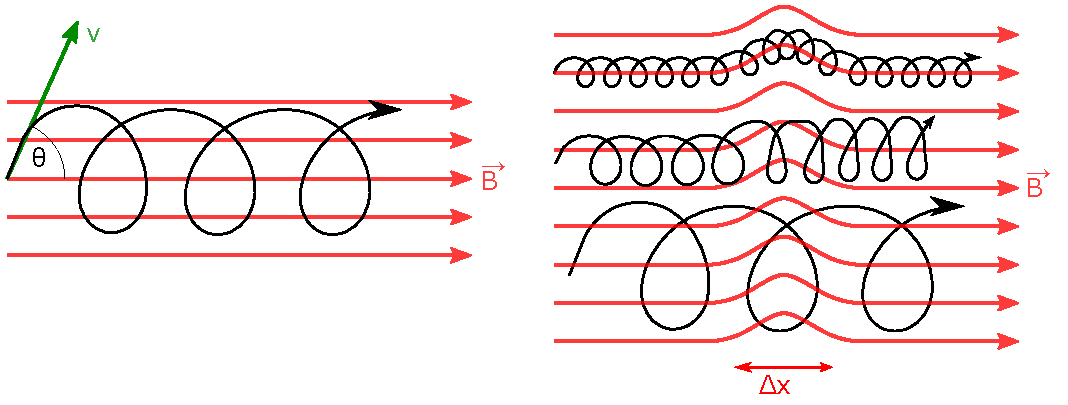
\includegraphics[width=1.0\textwidth]{04_Introduction/Images/cosmic_rays/combined_turbulence.pdf}
    \caption{ (\textit{left}) The path (black) of motion taken by a charged particle with initial velocity $v$ at angle $\theta$ to a uniform magnetic field $B$ (red). (\textit{right}) Propagation of a charged particle in a magnetic field  with turbulence of length $\Delta x$ when $r_g<\Delta x$ (\textit{top}), $r_g\approx \Delta x$ (\textit{middle}) and $r_g>\Delta x$. (\textit{bottom})}
    \label{fig:01_CR_in_Bfield}
\end{figure}

\noindent where $v_\perp$ is the velocity perpendicular to the magnetic field and $\hat{r}=\vec{r}/\abs{\vec{r}}$ represents the direction perpendicular both to the motion and the magnetic field. Combining \autoref{eq:chapter_1_lorentz_force} and \autoref{eq:chapter_1_centripetal_motion}, we find the particle gyro-radius, $r_g$ (the radius of the circular motion induced by a uniform magnetic field):

\begin{equation}
    \begin{aligned}
    r_g&=\frac{mv_\perp}{qB}=\frac{p}{qB}\text{ ,}
    \end{aligned} \label{eq:chapter_1_gyro-radius}
\end{equation}
\noindent where $p$ is the relativistic momentum of the charged particle. For relativistic cosmic rays $p\approx E/c$. If the charged particle has velocity at an angle $\theta$ to a magnetic field, it will spiral around the magnetic field direction as shown in the left panel of \autoref{fig:01_CR_in_Bfield}.
\newpar 
The magnetic field around PWNe and within dense gas clouds (see \autoref{eq:sec_Bfield_gas}) is not uniform and will affect the propagation of charged particles. The presence of magnetic field turbulence of length $\Delta x$ in an otherwise uniform field will affect the propagation of charged particles (see the right panel of \autoref{fig:01_CR_in_Bfield}). For charged particles, where the gyro-radius is much less than the magnetic turbulence ($r_g\ll \Delta x$), the particle will follow the magnetic field lines with no change to its pitch angle. When the gyro-radius is much greater than the turbulence ($r_g\gg \Delta x$), the propagation will be unaffected. For charged particles, where the gyro-radius is similar in scale to the perturbation ($r_g\approx \Delta x$), the pitch angle $\theta$ changes and alters the direction of travel. In other words, charged particles scatter on the magnetic field turbulence that is of similar scale as the gyro-radius.
\newpar
The gyro-radius of ultra-high energy particles ($r_g=3.6\,\kpc$ at $10^{19}\,\eV$ and $B=3\,\si{\micro G}$) is so large that they tend to travel in a ballistic manner (for distances less than $r_g$) and thus point back to their place of origin. Lower energy particles (e.g. $r_g\approx 10^{-4}\,\pc$ at $1\,\TeV$ and $B=3\,\si{\micro G}$) scatter multiple times and their trajectory tends to follow a random walk, i.e. diffusion.

\subsubsection{Diffusion of charged particles} 

The diffusion coefficient, $D\,\qty[\si{\centi\meter\squared\per\second}]$, describes the rate that charged particles diffuse across a unit area and is related to the magnetic field of the medium. In a magnetic field with average field strength $B_0$, the mean square variation $\delta B^2$ depends on the spatial power spectrum of the magnetic field turbulence $I\qty(k)\propto k^{-\Gamma}$ \citep{1983RPPh...46..973D,2016MNRAS.461.3552N}:

\begin{equation}
    \begin{aligned}
        \int I\qty(k) \dd{\ln k}&= \qty(\frac{\delta B}{B_0})^2\text{ ,}
    \end{aligned}
\end{equation}
\noindent where $k\propto 1/r_g$ is the wave number. As the charged particle spirals around the magnetic field lines (see \autoref{fig:01_CR_in_Bfield}), the pitch angle of the particle is changed by order $\delta B$. The pitch angle is randomised after approximately $N=B_0^2/kI\qty(k)$ rotations such that the mean free path parallel to the field is given by $\lambda_\parallel=Nr_g$. Therefore, the diffusion coefficient parallel to the magnetic field lines:

\begin{equation}
    \begin{aligned}
        D_\parallel&=\frac{r_gv}{3}\frac{B_0^2}{kI\qty(k)}\text{ ,}
    \end{aligned} \label{eq:01_diff_parallel}
\end{equation}
\noindent where $v$ is the velocity of the particle. The mean free path perpendicular to the field lines takes values $\lambda_\perp\approx r_g$ such that the perpendicular diffusion coefficient becomes:

\begin{equation}
    \begin{aligned}
        D_\perp&=\frac{r_gv}{3}\frac{kI\qty(k)}{B_0^2}=D_\parallel\qty(\frac{kI\qty(k)}{B_0^2})^2\text{ .}
    \end{aligned}
\end{equation}
\noindent Hence:

\begin{equation}
    \begin{aligned}
        D_\perp D_\parallel&=\qty(\frac{r_gv}{3})^2=D_B^2\text{ ,}
    \end{aligned}
\end{equation}
\noindent where $D_B=r_gv/3$ is known as the Bohm diffusion coefficient representing the case when $\lambda\approx r_g$.
\newpar 
Three different regimes of turbulence are considered: Bohm ($\Gamma=1$), Kraichnan ($\Gamma=\frac{3}{2}$) and Kolmogrov ($\Gamma=\frac{5}{3}$). Quasi-linear theory states that diffusion perpendicular to the magnetic field lines is negligible (\cite{2016MNRAS.461.3552N} and references within). As $r_g\propto E$ and $k\propto 1/E$, \autoref{eq:01_diff_parallel} becomes:

\begin{equation}
    \begin{aligned}
        D&\propto \frac{r_g}{kI\qty(k)}\propto E^{2-\Gamma} \text{ .}
    \end{aligned}
\end{equation}
This results in energy dependent diffusion: $D\propto E$ in the Bohm regime, $D\propto E^{\frac{1}{2}}$ in the Kraichnan regime and $D\propto E^{\frac{1}{3}}$ in the Kolmogrov regime. From cosmic-ray observations, values of the diffusion coefficient follows a power law spectrum ($D\propto E^{\delta}$) with $\delta$ taking values between $0.3-0.6$, implying a situation in the Kraichnan/Komogrov regime (e.g. see \cite{2007ARNPS..57..285S}).
\newpar 
Neglecting acceleration, \cite{2007Ap&SS.309..365G} parameterized the diffusion coefficient for cosmic rays of energy $E$ travelling in a molecular cloud with a magnetic field $B$ to be:
\begin{align}
    D\qty(E,B)&=\chi D_0\qty(\frac{E/\GeV}{B/3\,\si{\micro G}})^\delta\quad [\si{\centi\meter\squared\per\second}] \label{eq:diffusion}
\end{align}
where $D_0=1\times 10^{27}\,\si{\centi\meter\squared\per\second}$ is the Galactic diffusion coefficient at $1\,\GeV$ and the factor, $\chi$, takes values\,$<1$ and accounts for the suppression of the diffusion coefficient inside turbulent clouds \citep{1990acr..book.....B}. \cite{1996A&A...309..917A} consider $\chi=0.01$ to be `slow' diffusion representing dense ISM clouds \citep{1988ApJ...334..722O} and $\chi=1$ to be `fast' diffusion. The diffusion suppression factor is poorly constrained but studies towards SNR W28: \citep{2010MNRAS.409L..35L}, \citep{2010A&A...516L..11G} and \cite{2010sf2a.conf..313G} assume $\chi=0.1$, $0.01$ and $0.06$ respectively for $D_0=10^{28}\,\si{\centi\meter\squared\per\second}$ at cosmic-ray energy $10\,\GeV$. Similarly, \cite{2008MNRAS.390..683P} highlighted the variation of the suppression factor ($\chi=0.01$, $0.1$, $1$ and $\chi \gg 1$) in studies towards star forming region Sgr\,B2.

\subsubsection{Local and Galactic Magnetic Fields}

Magnetic fields affect the propagation of charged particles through the Galaxy. Faraday rotation (the rotation of polarised light in magnetised plasma) can be used to measure the magnetic field strength in the Galaxy \citep{1846RSPT..136....1F}:

\begin{equation}
    \begin{aligned}
    \langle B_\parallel \rangle = 1.232 \frac{\text{RM}}{\text{DM}}\text{ ,}
    \end{aligned}
\end{equation}
\noindent where $B_\parallel$ is the magnetic field component along the line of sight, RM is the rotation measure due to Faraday rotation and DM (see \autoref{eq:chapter_1_dispersion_measurement} is the dispersion measurement of the pulsar. Magnetic fields are also measured through observations of synchrotron emission, where the intensity is proportional to the magnetic field strength and electron energy density (see \cite{2013pss5.book..641B} and references within).
\newpar 
The magnetic field in the `local' vicinity takes value $1-6\,\si{\micro G}$ based on both rotation measure and synchrotron measurements  \citep{1989ApJ...343..760R,2001SSRv...99..243B}.  Using the rotation measures from $223$ pulsars, \cite{2006ApJ...642..868H} found the magnetic field strength in the Galactic disk was found to depend on the distance to the Galactic centre:

\begin{equation}
    \begin{aligned}
        B=B_0\exp[-\frac{R-R\odot}{R_B }]\text{ ,}
    \end{aligned}
\end{equation}
where $B_0=2.1\pm 0.3\,\si{\micro G}$ and $R_B=8.5\pm 4.7\,\kpc$. This gives the average Galactic magnetic field to be approximately $ 3\,\si{\micro G}$. Local sources such as PWN (see \autoref{sec:01_PWN}), SNRs (see \citep{2012SSRv..166..231R} and references within) and turbulent molecular clouds \citep{2010ApJ...725..466C} provide an `additional' magnetic field component to their surrounding environment.

\subsection{Cosmic-Ray Spectrum} \label{sec:chapter_1_cr_spectrum}
\begin{SCfigure}[0.4][b!]
    \centering
    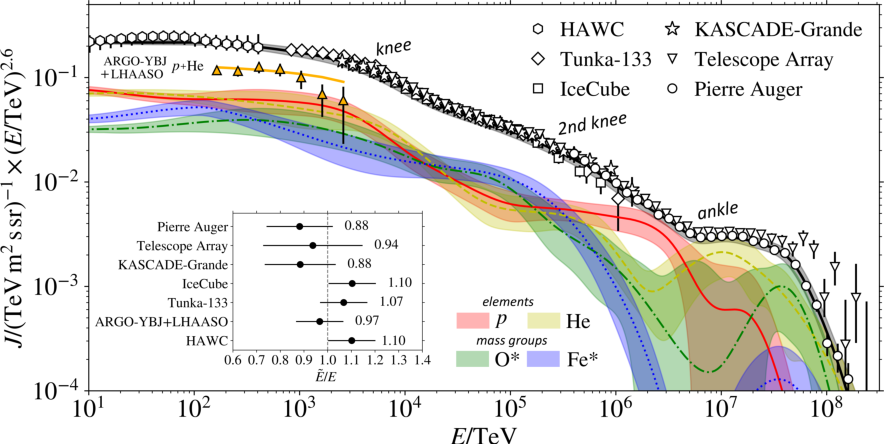
\includegraphics[width=0.75\textwidth]{04_Introduction/Images/cosmic_rays/cosmic_ray_spectrum.pdf}
    \caption{Cosmic-ray (and high-energy electron) energy spectrum at Earth as measured by multiple ground-based observatories. Image courtesy of \cite{2019BAAS...51c.131S}}
    \label{fig:chapter1_cosmic_ray_flux}
\end{SCfigure}
\newpar
The energy spectrum of cosmic rays (see \autoref{fig:chapter1_cosmic_ray_flux}) has been measured up to $10^{20}\,\eV$ \citep{2022arXiv221116020T} and broadly follows a power-law:

\begin{equation}
    \begin{aligned}
    \dv{N}{E}&\propto E^{-\Gamma}\text{ .}
    \end{aligned}
\end{equation}

Below $10\,\GeV$, the cosmic-ray energy spectrum is dominantly composed of high-energy particles originating from the Sun. Below this energy, there are few cosmic rays that originate from outside the solar system due to "frozen in" magnetic fields carried by the solar wind. Cosmic rays below $10\,\GeV$ have a gyro-radius (see \autoref{eq:chapter_1_gyro-radius}) smaller than the magnetic irregularities within this structure and are scattered out of the solar system \citep{2002cra..book.....S}. The cosmic-ray spectrum broadly follows a power law with spectral index $\Gamma\approx 2.7$ until the `knee' at $10^{15}\,\eV=1\,\PeV$ when it steepens to an index of $3$. Ground-based cosmic-ray detectors have reported a second knee at $10^{17}\,\eV$ where the spectrum steepens further to $3.3$ until it flattens out to $\approx 2.6$ at the ankle ($10^{18}\,\eV=1\,\si{E\electronvolt}$) \citep{2008ApJ...678.1165A,2010PhLB..685..239A, 2013PhRvD..87h1101A, 2013PhRvD..88d2004A,2013ApJ...768L...1A}. The knee and ankle feature is believed to be created due to the transition of Galactic cosmic rays (from sources such as SNRs and PWNe) to extra-Galactic cosmic rays, possibly originating from AGN \citep{2016A&A...595A..33T}. The cosmic-ray spectrum then experiences a sharp cutoff at $29\times10^{18}\,\eV = 29\,\si{E\electronvolt}$ due to the GKZ cutoff, where cosmic-ray protons and nuclei interact with the CMB and rapidly lose their energy \citep{1966PhRvL..16..748G,1966JETPL...4...78Z}. 

\subsection{PeVatrons} \label{sec:chapter_1_PeVatrons}
\begin{table}[h!]
    \caption{Observed HAWC and LHAASO sources with significant gamma-ray emission greater than $100\,\TeV$
    \citep{PhysRevLett.124.021102,2021Natur.594...33C}. The sources associated with \mbox{HESS\,J1825-137} are highlighted in blue.}
    \label{tab:chapter1_peVatron_candidates}
    \resizebox{\textwidth}{!}{
    \begin{threeparttable}
    \centering
   \begin{tabular}{ccccc}
        \hline
         & \textbf{Source} & \textbf{$\TeV$ counterpart$^*$} & \textbf{Accelerator$^*$} & $\sqrt{\text{TS}}$ \\
         \hline
         \textbf{HAWC} &  & & & \\
         & \textcolor{blue}{eHWC\,J1825-134} & \textcolor{blue}{\mbox{HESS\,J1825-137}, \mbox{HESS\,J1826-130}} & \textcolor{blue}{PWN} & \textcolor{blue}{$41.1$} \\
         & eHWC\,J1907+063 & HESS J1908+063 & Unidentified & $37.8$ \\
         & eHWC\,J2019+368 & 2HWC J2019+367 & Possible PWN$^{a}$ & $32.2$ \\
         \textbf{LHAASO} & & & & \textbf{Significance} \\
         & & & & $>100\,\TeV (\times \sigma)$ \\
         & LHAASO J0534+2202 & Crab Nebula & PWN & $17.8$ \\
         & \textcolor{blue}{LHAASO J1825-1326} & \textcolor{blue}{HESS J1825-137} & \textcolor{blue}{PWN} & \textcolor{blue}{$16.4$} \\
         & LHAASO J1839-0545 & HESS J1837-069 & Possible PWN & $7.7$ \\
         & LHAASO J1843-0338 & HESS J1843-033, HESS J1844-030, & Possible SNR & $8.5$ \\
         & & SNR G28.6-0.1 & & \\
         & LHAASO J1849-0003 & HESS J1849-000, W43W  & Possible PWN$^{b}$ & $10.4$ \\
         & LHAASO J1908+0621 & HESS J1908+063, MGRO J1908+06 & Possible SNR or PWN & $17.2$ \\
         & LHAASO J1929+1745 & HESS J1930+188 & Possible PWN or SNR & $7.4$ \\
         & LHAASO J1956+2845 & 2HWC J1955+285, SNR G66.0-0.0 & Possible PWN SNR & $7.4$ \\
         & LHAASO J2018+3651 & MGRO J2019+37  & Possible PWN & $10.4$ \\
         & LHAASO J2032+4102 & - & Possible PWN & $10.5$ \\
         & LHAASO J2108+5157 & - & Possible PWN & $8.3$ \\
         & LHAASO J2226+6057 & Boomerang Nebula & Possible SNR or PWN & $13.6$ \\
         \hline
    \end{tabular}
    \begin{tablenotes}
	\item $^*$: Counterparts are based on spatial correlation.  \\
	\textbf{References}
	\item $^{a}$ \cite{2018APS..APRB17003B} 
	\item $^{b}$ \cite{2015MNRAS.449.3827K} 
    \end{tablenotes}
    \end{threeparttable}
    }
\end{table}
The transition from Galactic to extra-Galactic cosmic rays in the cosmic-ray spectrum occurs between $10^{15}\,\eV$ and $10^{18}\,\eV$ with Galactic cosmic rays expected to contribute up to $10^{17}\,\eV=100\,\PeV$ \citep{2016A&A...595A..33T}. Sources capable of accelerating particles up to and beyond $1\,\PeV=10^{15}\,\eV$ are known as PeVatrons. Finding Galactic PeVatrons is key to understanding the mechanism of accelerating particles up to $\PeV$ energies.
\newpar
Cosmic rays with energies $1\,\PeV$ and $100\,\PeV$ have gyro-radii of $\approx 0.4\,\pc$ and $40\,\pc$ respectively, making their direct origin impossible to determine. However, cosmic rays interact with interstellar gas and magnetic fields near their birthplace to produce gamma rays with energies greater than $100\,\TeV$ (see \autoref{sec:chapter1_non_thermal_emission}). Therefore, any gamma-ray source with significant gamma-ray emission above $100\,\TeV$ is an indicator of a PeVatron
\newpar 
The High-Altitude Water Cherenkov Gamma-ray observatory (HAWC) and the Large High Altitude Air Shower observatory (LHAASO) are observatories that detect particle showers triggered by gamma rays \citep{LHAASO_website, HAWC}. \autoref{tab:chapter1_peVatron_candidates} lists observed HAWC and LHAASO sources with significant gamma-ray emission above $100\,\TeV$ with possible counterparts and accelerator type \citep{PhysRevLett.124.021102,2021Natur.594...33C}. In the past, SNRs have been regarded as the most likely source capable of accelerating protons up to $\PeV$ energies. However, there has been no firm identification of a SNR PeVatron and their suitability as a PeVatron has been called into question \citep{10.1093/mnras/sty1589,2019IJMPD..2830022G,2021Univ....7..324C,2022MNRAS.516..492B}. However, both the Crab Nebula and \mbox{HESS\,J1825-137} are the confirmed $\TeV$ PWN counterparts of \mbox{LHAASO\,J0534+2202} and \mbox{LHAASO\,J1825-1326} respectively. Out of the remaining LHAASO candidates, at least eight have possible PWN counterparts. PWN are now being considered as possible candidates to accelerate electrons up to $\PeV$ energies \citep{2021ApJ...908L..49B,de_O_a_Wilhelmi_2022}. \cite{2022ApJ...928...19V} suggests that unresolved PWNe provides significant contribution to the diffuse gamma-ray emission above $100\,\TeV$.
\newpar
H.E.S.S. has only discovered one PeVatron that is postulated to be associated with the black hole in the Galactic Center during an active phase \citep{2016Natur.531..476H}. They highlighted that the current rate of its particle acceleration is not powerful enough to explain the cosmic-ray flux at Earth.  Alternatively, superbubbles and massive stellar clusters have been proposed as PeVatron candidates. Stellar clusters form within dense molecular clouds, creating an expanding `bubble' of low density ISM \citep{1998LNP...506..399I}. It has been suggested that turbulent plasma within superbubbles confine cosmic rays, allowing multiple shock fronts to accelerate them to high energies (e.g. see \cite{2022MNRAS.515.2256V} and references within).
\newpar 
The \mbox{Tibet AS$\gamma$} collaboration revealed the detection of diffuse gamma rays with energies between $100\,\TeV$ to $10^3\,\TeV=1\,\PeV$ in the Galactic disk, indicating the presence of PeVatrons in the Galaxy \citep{PhysRevLett.126.141101}. Similarly, LHAASO reported measurements of the diffuse gamma-ray emission up to $1000\,\PeV$ and suggests that $\TeV$ halos (see \autoref{sec:01_intro_time_ev_PWN}) significantly contribute to the diffuse emission up to the ultra-high energy band \citep{2023arXiv230505372C}.

\section{Gamma rays: Messengers of Cosmic Rays} \label
{sec:chapter1_non_thermal_emission}
\autoref{chapter_1_cr_propagation} and \autoref{sec:chapter_1_PeVatrons} discussed how Galactic cosmic rays ($E<100\,\PeV$) scatter off magnetic field turbulence and do not preserve information about their origin. Therefore, alternate messengers for Galactic cosmic rays must be turned to. Gamma rays are produced via hadronic (cosmic-ray proton) and leptonic (cosmic-ray electron) interactions with the ISM and/or radiation fields. This section will describe the history of gamma-ray astronomy and then delve deeper into their production processes.

\subsection{A Brief History}

Gamma rays were first discovered in 1900 by Paul Villard while studying radium. Ernest Rutherford later realised in 1903 that this radiation was fundamentally different to alpha, beta and delta rays and subsequently classified them as gamma rays. By reflecting gamma rays from a crystal surface, Rutherford and Edward Andrade in 1913 proved the electromagnetic nature of gamma rays and measured their wavelength \citep{1913Natur..92..267R}. Gamma rays have the largest energy per photon and smallest frequency of the electromagnetic spectrum. On Earth, gamma rays are created by radioactive decay within the crust and the interaction of cosmic rays with the Earth's atmosphere. Gamma-ray astronomy began with the 1957 publication by Philip Morrison, with the prediction that solar flares produce gamma rays \citep{1958NCim....7..858M}. We now know of many astrophysical sources that can produce gamma rays. These include PWNe, SNRs, quasars and active Galactic nuclei. Current gamma-ray observatories include \textit{Fermi} Gamma-ray Space Telescope \citep{nasa_fermi_site}, the High Energy Stereoscopic System \citep{HESS}, MAGIC \citep{MAGIC}, HAWC \citep{HAWC}, VERITAS \citep{VERITAS} and LHAASO \citep{LHAASO_website}. Details of gamma-ray detection will be discussed in \autoref{sec:02_astronomy}.

\subsection{Hadronic Gamma-Ray Emission} \label{sec:chapter1_hadronic_gr_emission}

Relativistic protons (and nuclei) collide with gas in the ISM to form charged and neutral pions via proton-proton (p-p) interactions:

\begin{equation}
    \begin{aligned}
    p+p&\rightarrow \pionneutral + \pionplus + \pionminus
    \end{aligned}
\end{equation}
\noindent During p-p interactions, about half of the energy of the initial cosmic-ray proton is split among the neutral and charged pions  \citep{2009ARA&A..47..523H}. The subsequent decay of neutral pions produce gamma rays:

\begin{equation}
    \begin{aligned}
    \pionneutral & \rightarrow \gamma +\gamma
    \end{aligned}
\end{equation}
\noindent with each gamma ray carrying approximately one sixth of the initial proton energy \citep{2009ARA&A..47..523H}. The charged pions decay into muons, neutrinos and anti-neutrinos:

\begin{equation}
    \begin{aligned}
    \pionplus &\rightarrow \muonplus + \muonneutrino \\
    \pionminus &\rightarrow \muonminus + \antimuonneutrino
    \end{aligned}
\end{equation}
\noindent Similarly, muons go on to decay into electrons, positions, neutrinos and anti-neutrinos:

\begin{equation}
    \begin{aligned}
    \muonminus &\rightarrow e^- + \bar{\nu}_e+\nu_\mu \\
    \muonplus &\rightarrow e^+ + \nu_e + \bar{\nu}_\mu
    \end{aligned}
\end{equation}
\begin{figure}[b!]
    \centering
    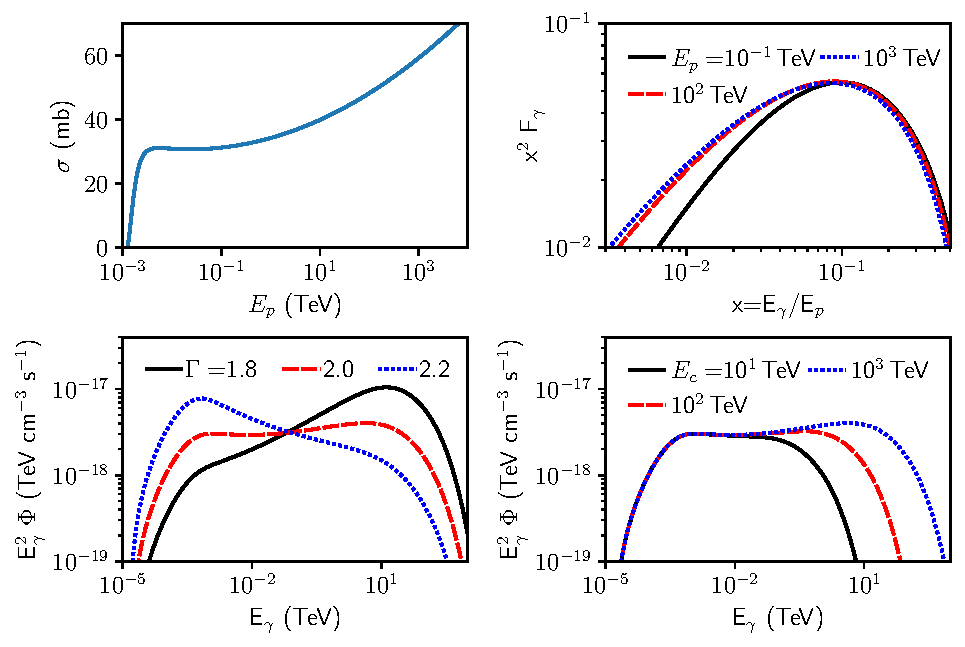
\includegraphics[width=\textwidth]{04_Introduction/Images/non_thermal_emission/hadronic_interaction.pdf}
    \caption{(\textit{top-left}) Proton-proton interaction cross section as given by \autoref{eq:chapter1_non_thermal_pp_cross_section}. (\textit{top-right}) Hadronic gamma-ray emission from a cosmic-ray proton with energy $E_p$ and target density $n_H=1\,\centimeterminusthree$ (\textit{bottom}) Gamma-ray spectra from p-p interactions from cosmic-rays protons with an exponential cutoff power law distribution ($\dd{N}/\dd{E}\propto E^{-\Gamma}\exp(-E/E_c)$) with $E_c=10^3\,\TeV$ (\textit{left}) and $\Gamma=2.0$ (\textit{right}).}
    \label{fig:chapter_1_non_thermal_hadronic_emission}
\end{figure}
\newpar
For a distribution of protons with spectral index $\Gamma$ and exponential cutoff energy $E_c$:

\begin{equation}
    \begin{aligned}
    J_P\qty(E_p) &= A E_p^{-\Gamma} \exp(-\frac{E_p}{E_C})\quad\qty[\si{\per\tera\electronvolt\per\centi\meter\cubed}]\text{ ,}
    \end{aligned}
\end{equation}
\noindent where $A$ is a normalisation constant, the energy spectra of gamma rays from proton-proton collisions is expected to follow:

\begin{equation}
    \begin{aligned}
	\Phi\qty(E_\gamma)&=\dv{N_\gamma}{E_\gamma}=cn_H\int_{E_\gamma}^\infty\sigma_{pp}\qty(E_p)J_p\qty(E_p)F_\gamma\qty(T_p,E_\gamma)\frac{\dd{E_p}}{E_p}\text{ ,}
\end{aligned} \label{eq:01_hadronic_g_spectrum}
\end{equation}
\noindent where $c$ is the speed of light and $n_H$ is the density of the ambient medium.
From the bottom panels in \autoref{fig:chapter_1_non_thermal_hadronic_emission} it can be seen that the shape of the p-p gamma-ray SED is influenced by the distribution of cosmic-ray protons. While the spatial morphology of hadronic gamma rays is shaped by interstellar gas, as seen in \autoref{eq:01_hadronic_g_spectrum}. In summary, gamma rays act as messengers for hadronic cosmic rays and carry information about the source and its surrounding environment.
\newpar
The total inelastic cross section of p-p interactions for a proton of kinetic energy $T_p$ (where the total energy is $E_p=m_pc^2+T_p$) is given by \citep{2014PhRvD..90l3014K}:

\begin{equation}
    \begin{aligned}
    \sigma_{pp}\qty(T_p) &= \qty(30.7-0.96\ln\qty(\frac{T_p}{T_\text{thr}})+0.18\ln^2\qty(\frac{T_p}{T_\text{thr}}))\qty(1-\qty(T_\text{thr}/T_p)^{1.9})^3\quad\qty[\si{\milli\barn}]\text{ ,}
    \end{aligned} \label{eq:chapter1_non_thermal_pp_cross_section}
\end{equation}
\noindent where $T_\text{thr}=2m_\pi + m_\pi^2/2m_p \approx 0.28\,\GeV$ is the minimum proton kinetic energy to form a neutral pion ($E_\text{thr}=1.22\,\GeV$). The top-left panel of \autoref{fig:chapter_1_non_thermal_hadronic_emission} shows the total inelastic cross section at different proton energies.
\newpar
The time it takes for a proton to lose its energy (or `cool' to a lower energy) through p-p interactions in a medium with ambient density $n_H$ is given by \citep{2009ARA&A..47..523H}:

\begin{equation}
    \begin{aligned}
	\tau_{pp} &= \frac{1}{nc\kappa\sigma_{pp}\qty(E)} \\
	&\approx 5.3\times 10^7\qty(n/\centimeterminusthree)^{-1}\quad\qty[\si{yr}]\text{ .}
\end{aligned} \label{eq:chapter_1_pp_cooling time}
\end{equation}
\noindent \autoref{eq:chapter_1_pp_cooling time} shows that the cooling rate of protons is inversely proportional to the density of interstellar gas and approximately independent of the proton energy. Therefore, the brightness of gamma rays towards a source of cosmic-ray protons will correlate with the density morphology of the surrounding ISM gas.
\newpar 
Using GEANT4 models, \cite{2014PhRvD..90l3014K} parameterized the spectra of gamma rays of energy ($E_\gamma$) from a single proton with kinetic energy $T_p$ to be:

\begin{equation}
    \begin{aligned}
        F_\gamma\qty(T_p, E_\gamma)&= A_\text{max}\qty(T_p) F\qty(T_p, E_\gamma) \text{ ,}
    \end{aligned} \label{eq:chapter_1_non_thermal_hadronic_flux_single_proton}
\end{equation}
\noindent where $A_\text{max}$ is a function of the pion production and $F\qty(T_p, E_\gamma)$ describes the shape of the spectrum:

\begin{subequations}
	\begin{alignat}{2}
		A_\text{max}\qty(T_p) &=\sigma_\pi\qty(T_p)
        \begin{cases}
        {b_0}/{E_\pi^\text{max}}&\text{, } T_\text{thr}\leq T_p < 1\,\GeV \\
        {b_1\theta_p^{-b_2}}/{m_p}\times \exp(b_3\ln^2\theta_p) &\text{, } T_p \geq 1\,\GeV \\
        \end{cases} \\
        F_\gamma \qty(T_p, E_\gamma)&=\frac{\qty(1-X_\gamma^{\alpha\qty(T_p)})^{\beta\qty(T_p)}}{\qty(1+X_\gamma/C)^{\gamma\qty(T_p)}}\text{ ,}
	\end{alignat}
\end{subequations}
\noindent with $\sigma_\pi$ being the $\pi_0$ production cross section (see \cite{2014PhRvD..90l3014K} for parameterisation), $\theta_p=T_p/m_p$, $E_\pi^\text{max}$ is the maximum total $\pi_0$ energy in the laboratory frame, $C=\lambda  m_\pi/Y_\gamma^\text{max}$, $Y_\gamma=E_\gamma+m_\pi^2/\qty(4E_\gamma)$, $X_\gamma=(Y_\gamma-m_\pi)/(Y_\gamma^\text{max}-m_\pi)$ and $b_0=5.9$, $b_1$, $b_2$, $b_3$, $\alpha\qty(T_p)$, $\beta\qty(T_p)$, $\gamma\qty(T_p)$ and $\lambda$ are coefficients for the GEANT4 modelling (see \autoref{A6_misc}). The top-right panel of \autoref{fig:chapter_1_non_thermal_hadronic_emission} shows the expected gamma-ray spectra from a proton with energy $E=0.1\,\TeV$, $100\,\TeV$ and $1000\,\TeV$.

\subsection{Leptonic Gamma-Ray Emission} \label{sec:chapter_1_leptonic_gre}

Cosmic-ray electrons produce $\GeV$ to $\TeV$ gamma rays through synchrotron, inverse Compton and Bremsstrahlung interactions.

\subsubsection{Synchrotron Radiation}

Synchrotron radiation occurs when charged particles gyrate in a magnetic field of strength $B$. For a particle with mass $m$, charge $q$ and Lorentz factor $\gamma$, the angular velocity is given by:

\begin{equation}
    \begin{aligned}
    	\omega &=\frac{qB}{\gamma m}\text{ .}
    \end{aligned}
\end{equation}
\noindent The total power radiated by a charged particle is given by Larmor's formula:

\begin{equation}
    \begin{aligned}
    P=\frac{q^2a^2}{6\pi\epsilon_0c^3}\quad\qty[\si{\ergs\per\second}]\text{ ,}
    \end{aligned}
\end{equation}
\noindent where $a$ is the acceleration of the particle.

\begin{figure}[b!]
	\centering
	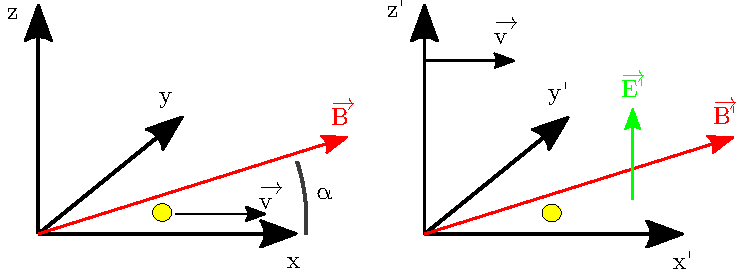
\includegraphics[width=0.7\textwidth]{04_Introduction/Images/non_thermal_emission/synchrotron_frames.pdf}
	\caption {An electron travelling at velocity $\vec{v}$ in the x-direction of the lab frame (\textit{left}) with a uniform magnetic field on the x-y plane at angle $\alpha$ to the x-axis. The rest frame of the particle (\textit{right}) travels at velocity $\vec{v}$ to the lab frame. The pure magnetic field $\vec{B}$ (i.e. no electric fields) in the lab frame appears as a mixture of magnetic field $\vec{B}'$ and electric field $\vec{E}'$ in rest frame.}
	\label{fig:chapter_1_non_thermal_sync_frames}
\end{figure}
\newpar 
In the rest frame of the ($\vec{v}=0$), the force acted on the particle is described by:

\begin{equation}
	\begin{split}
		\vec{F}&=m\vec{a}=-e\qty(\vec{E}+\vec{v}\times \vec{B})  \\
		&=-e\vec{E}\text{ ,}
	\end{split}
\end{equation}
where $\vec{E}$ is the electric field strength in the particle's rest frame. For the example shown in \autoref{fig:chapter_1_non_thermal_sync_frames}, the parallel and perpendicular component of the electric field in the particle's rest frame can be obtained using Lorentz transformations:

\begin{subequations}
	\begin{align}
		\vec{E}_\parallel'&=\vec{E}_\parallel=0 \\
		\vec{E}_\perp'&=\gamma\qty(\vec{E}_\perp +\vec{v}\times \vec{B}_\perp) = E_z' = \gamma vB\sin\alpha\text{ .}
	\end{align}
\end{subequations}
\noindent Therefore the power radiated is given by:

\begin{equation}
    \begin{aligned}
	P&=-\frac{\qty(\gamma evB\sin\alpha/m)^2e^2}{6\pi\epsilon_0c^3}\text{ ,}
    \end{aligned} \label{eq:chapter_1_non_thermal_sync_power}
\end{equation}
\noindent where the negative in \autoref{eq:chapter_1_non_thermal_sync_power} represents the energy lost by the particle. Power is Lorentz invariant, hence \autoref{eq:chapter_1_non_thermal_sync_power} applies to both the lab and rest frame in \autoref{fig:chapter_1_non_thermal_sync_frames}. Electrons radiate more power via synchrotron radiation than protons of the same energy due to the inverse proportionality of the particle's mass (see \autoref{eq:chapter_1_non_thermal_sync_power}). Henceforth, only synchrotron radiation from electrons will be considered. The power radiated by a single electron through synchrotron radiation is:

\begin{equation}
    \begin{aligned}
    P&=-2\sigma_T\gamma^2c U_B\sin^2\alpha\text{ ,}
    \end{aligned}
\end{equation}
\noindent with the magnetic energy density defined to be $U_B=B^2/2\mu_0$ and the Thompson cross section is defined as:

\begin{equation}
    \begin{aligned}
    \sigma_T&=\frac{8\pi}{3}\qty(\frac{e^2}{4\pi\epsilon_0m_ec^2})^2=\frac{8\pi}{3}r_0^2\text{ ,}
    \end{aligned}
\end{equation}
\noindent where $r_0={e^2}/{4\pi\epsilon_0m_ec^2}$ is the classical electron radius. For electrons travelling in random directions:

\begin{equation}
    \begin{aligned}
        \left\langle \sin^2\alpha \right\rangle&=\half \int_{-1}^1\sin^2\alpha\dd{\cos\alpha}=\frac{2}{3}\text{ .}
    \end{aligned}
\end{equation}
\noindent The mean power loss is given by:

\begin{equation}
    \begin{aligned}
    \left\langle P\right\rangle&=\dv{E}{t}=-\frac{4}{3}\sigma_T\gamma^2 c U_B\text{ .}
    \end{aligned} \label{eq:01_leptonic_sync_energy_loss}
\end{equation}

The spectrum, $P\qty(\nu)$, of synchrotron emission emitted by a single electron with pitch angle $\alpha$ and magnetic field $B$ is given by \citep{2007A&A...474..689M}:

\begin{equation}
    \begin{aligned}
    j \qty(\nu)&=\dv{N}{E}=\frac{\sqrt{3}e^3B\sin\alpha}{mc^2}\frac{\nu}{\nu_c}\int_{x=\nu/\nu_c}^{\infty}K_\frac{5}{3}\qty(t)\dd{t}\text{ ,}
    \end{aligned} \label{eq:01_nontherm_sync_indiv}
\end{equation}
\begin{SCfigure}[0.42][h!]
    \centering
    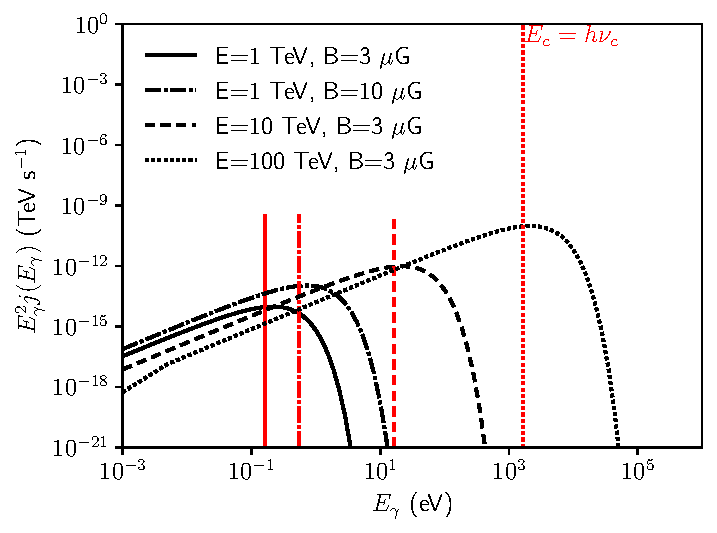
\includegraphics[width=0.7\textwidth]{04_Introduction/Images/non_thermal_emission/synchrotron_spectrum.pdf}
    \caption{Synchrotron emission from an electron with energy $E$ in magnetic field $B$. The red vertical lines represent the equivalent critical energy ($E_c=h\nu_c$).}
    \label{fig:01_sync_flux}
\end{SCfigure}
\noindent where $K_\frac{5}{3}$ is the modified Bessel function of the second kind. The synchrotron spectrum, $P\qty(\nu)$, peaks at `critical frequency' $\nu=\nu_c$ (see \autoref{fig:01_sync_flux}):
\begin{equation}
    \begin{aligned}
    \nu_c&=\gamma^2\frac{3eB\sin\alpha}{4\pi mc}\text{ .}
    \end{aligned}
\end{equation}
\noindent Equivalently, the synchrotron spectrum peaks at photon energy $E_\gamma$ \citep{2009ARA&A..47..523H}:

\begin{equation}
    \begin{aligned}
    \frac{E_\gamma}{\eV}&=0.087 \qty(\frac{E_e}{\TeV})^2 \frac{B}{\si{\micro G}}\text{ ,}
    \end{aligned}
\end{equation}
\noindent where $E_e$ is the energy of the initial electron. Therefore, observations of synchrotron emission $\gtrsim 300\,\keV$ is a strong indicator of a source accelerating electrons up to $\PeV$ energies.

\subsubsection{Inverse Compton emission}

Inverse Compton emission occurs when an electron scatters off a photon:

\begin{align}
	\gamma_\text{low E} + e^{-'}&\rightarrow \gamma_{\TeV}+e^{-}\text{ ,}
\end{align}
where the final photon energy is greater than the original photon energy at cost of the electron energy ($E_{e^{-'}}>E_{e^-}$). Photon fields such as the CMB, infra-red photons, visible light, UV and X-rays provide target photons for the electron to scatter up to $\gamma$-ray energies. 
\newpar
\begin{figure}[h!]
	\centering
	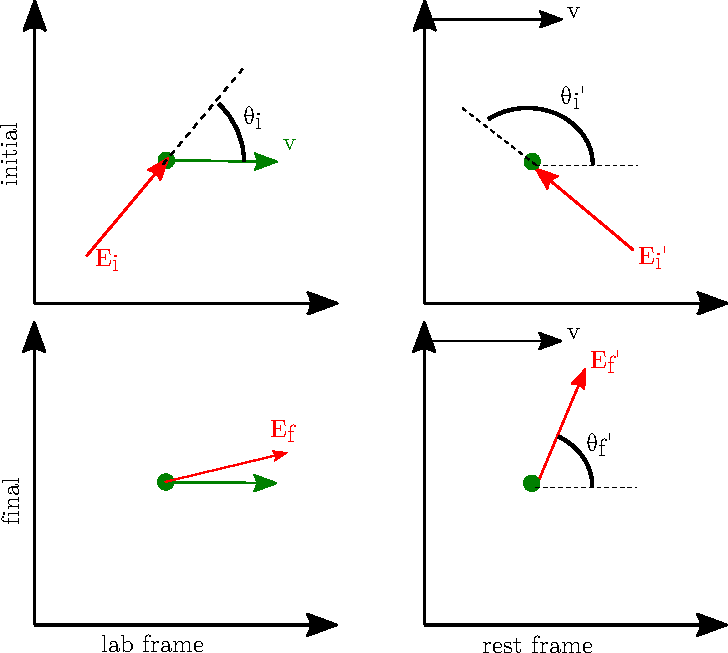
\includegraphics[width=0.7\textwidth]{04_Introduction/Images/non_thermal_emission/inverse_compton.pdf}
	\caption{A photon with energy $E_i$ scatters of an electron (travelling at velocity $v$) at angle $\theta$ in the lab frame (\textit{left}). In the rest frame of the electron (\textit{right}), the photon collides with electron at angle $\theta'$ and energy $E_i'$. The top and bottom panels describe the situation before and after the collision respectively. After scattering the photon has energy $E_f$ and $E_f'$ in the lab frame and electron rest frame respectively}
	\label{fig:chapter_1_non_thermal_compton_rest_frames}
\end{figure}
\autoref{fig:chapter_1_non_thermal_compton_rest_frames} shows a photon with momentum $\qty[\frac{E_i}{c},\frac{E_i}{c}\cos\theta_i,\frac{E_i}{c}\sin\theta_i,0]$ scattering off an electron in the lab and rest frame of the electron. The Lorentz transformation of the initial photon energy from the lab frame ($E_i$) to the rest frame ($E_i'$) is given by:

\begin{equation}
    \begin{aligned}
        E_i'&=\gamma E_i\qty(1-\beta \cos\theta_i)\text{ ,}
    \end{aligned}    
\end{equation}
\noindent where $\beta = v/c$ and $v$ is the electron velocity. The Lorentz transformation of the final photon energy from the rest frame to the lab frame is given by:

\begin{equation}
	\begin{aligned}
		E_f&=\gamma E_f'\qty(1+\beta\cos\theta_f')\text{ .}
    \end{aligned}
\end{equation}
\noindent Assuming elastic scattering, the photon has the same energy before and after the collision in the rest frame of the electron ($E_i'=E_f'$). Therefore, the final energy in the lab frame is:

\begin{equation}
    \begin{aligned}
		E_f&=\gamma^2E_i\qty(1-\beta\cos\theta_i)\qty(1+\beta\cos\theta_f')\text{ .}
	\end{aligned}
\end{equation}
\noindent The photon scatters of the electron isotropically ($i.e.\left\langle\cos\theta_f'\right\rangle\approx 0$):

\begin{equation}
    \begin{aligned}
    \left\langle E_f\right\rangle&=\qty(1-\beta\cos\theta_i)\gamma^2 E_i\text{ .}
    \end{aligned}
\end{equation}
\noindent The rate of interaction, $R$, for electrons in photon field with density $n$ at angle $\theta_i$ can be described by:

\begin{equation}
    \begin{aligned}
    R&=n\sigma_T\qty(1-\beta\cos\theta_i)\text{ ,}
    \end{aligned}
\end{equation}
\noindent where $\sigma_T$ is the Thompson cross section. The rate of electron energy loss over a solid angle $\dd{\Omega}=2\pi\sin\theta_i\dd{\theta}=2\pi\,\dd{\qty(\cos\theta_i)}$ is given by:

\begin{equation}
	\begin{split}
		\dv{E}{t}&=-\frac{\dd{\Omega}}{4\pi}Rc\left\langle E_f\right\rangle \\
		&=-nE_i\sigma_T c\gamma^2\frac{\dd{\cos\theta}}{2}\qty(1-\cos\theta_i)^2\text{ .}
	\end{split}
\end{equation}
\noindent Integrating over all $\theta_i$ gives the electron energy loss for Inverse Compton Interactions as:

\begin{equation}
    \begin{aligned}
    \dv{E_e}{t}&=-\frac{4}{3}U_\text{rad}\sigma_T c\gamma^2 \text{ ,}
    \end{aligned}   \label{eq:chapter_1_non_thermal_IC_e_energy_lost}
\end{equation}
\noindent where $U_\text{rad}=n\qty(E_i)E_i$ is the radiation energy density and $n\qty(E_i)$ is the number density.
\newpar
The number density of target photons provided by photon fields such as the CMB can be described by a blackbody spectrum (see \autoref{sec:06_blackbodies}). Therefore, the spectrum from a single electron with energy $E_e$ scattering of a target photon with energy in range $\epsilon + \dd{\epsilon}$ is described by \citep{RevModPhys.42.237}:

\begin{equation}
    \begin{aligned}
        \frac{\dd{N}}{\dd{E_\gamma}}&=\frac{3\sigma_T mc^3}{4\gamma}\int_{E_\gamma/4\gamma^2}^{E_\gamma}\frac{n\qty(\epsilon)\dd{\epsilon}}{\epsilon}f\qty(q,\Gamma) \\
        f\qty(q,\Gamma)&=2q\ln q +\qty(1+2q)\qty(1-q)+\half\frac{\qty(\Gamma q)^2}{1+\Gamma q}\qty(1-q)\text{ ,}
    \end{aligned} \label{eq:01_nonthermal_IC_indiv_spectral}
\end{equation}
\noindent where:

\begin{subequations}
    \begin{align}
        q&=\frac{E_\gamma}{\Gamma\qty(E_e-E_\gamma)} \\
        \Gamma&=\frac{4\epsilon\gamma}{m_ec^2}\text{ .}
    \end{align}
\end{subequations}
\noindent $\Gamma$ determines whether the scattering falls under the Thompson limit ($\Gamma \ll 1$) or Klein-Nishina limit ($\Gamma \gtrsim 1$). The Thompson limit applies when the product of the incident and scattered photon energy is much less than the square of the rest mass of the electron \citep{RevModPhys.42.237}. The Klein-Nishina limit  takes in account the suppression of inverse Compton scattering for relativistic electrons.
\begin{SCfigure}[0.42][b!]
    \centering
    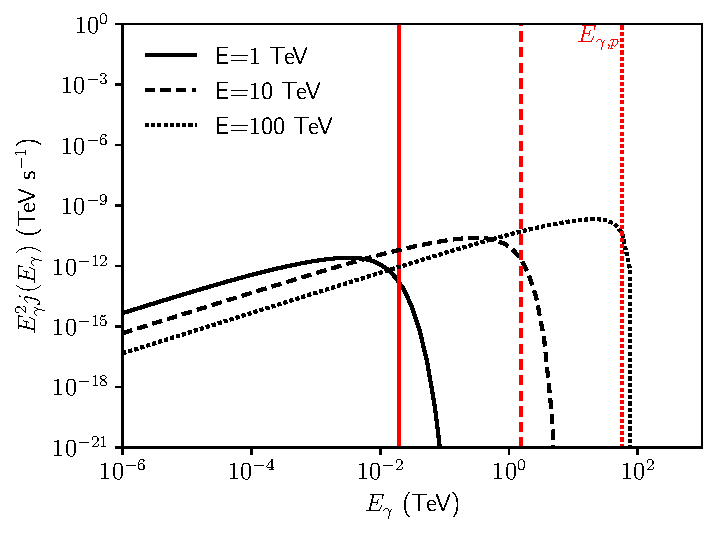
\includegraphics[width=0.7\textwidth]{04_Introduction/Images/non_thermal_emission/IC_spectrum.pdf}
    \caption{IC spectrum from an electron of energy $E$ interacting with the CMB.  The red vertical lines represent the energy at which the inverse Compton emission approximately peaks assuming a CMB photon has energy $\approx 7\times 10^{-4}\,\eV$.}
    \label{fig:01_IC_flux}
\end{SCfigure}
\newpar
In the Thompson regime, the inverse Compton emission peaks at \citep{2009ARA&A..47..523H}:

\begin{equation}
	\begin{split}
		\frac{E_{\gamma,p}}{\TeV}&\approx \frac{E_e}{\TeV}\frac{2.1b}{\qty(1+\qty(2.1b)^{0.8})^{1/0.8}} \\
		b&\approx 15\frac{E_e}{\TeV}\frac{\epsilon}{\eV}\text{ .}
	\end{split} \label{eq:01_non_thermal_IC_max}
\end{equation}
\noindent \autoref{eq:01_non_thermal_IC_max} is used to approximate the energy range of the cosmic-ray electron population. In the Klein-Nishina regime, \cite{doi:10.1126/science.abg5137} makes the approximation:

\begin{equation}
    \begin{aligned}
    \frac{E_e}{\PeV}&=2.15 \qty(\frac{E_{\gamma,p}}{\PeV})^{0.77}\text{ ,}
    \end{aligned}
\end{equation}
which is accurate to within $10\%$ for electrons within energy range $[30\,\TeV,3\,\PeV]$. Therefore, observations of gamma rays with energy $\gtrsim 200\,\TeV$ from inverse Compton interactions is a strong indicator that the source is a leptonic PeVatron (see \autoref{sec:chapter_1_PeVatrons}).

\subsubsection{Bremsstrahlung Emission}

Bremsstrahlung emission occurs when an electron experiences deacceleration due to the presence of an atomic nucleus. For a single electron with energy $E_e$ passing through a gas with number density $n$, the radiated photon spectrum per electron can be described by \citep{RevModPhys.42.237}:

\begin{equation}
	\begin{split}
		\frac{\dd{N}}{\dd{t}\dd{k}}&=cn\dd{\sigma} \text{ ,}
	\end{split} \label{eq:chapter_1_non_thermal_brem_SED}
\end{equation}
\noindent For an electron with initial \& final energy, $E_i$ \& $E_f$ respectively, the final photon has energy $k=E_i-E_f$. The differential cross section, $\dd{\sigma}$, can be written as \citep{1934RSPSA.146...83B}:

\begin{equation}
	\begin{split}
		\dd{\sigma}&=\alpha r_0^2\qty(\frac{\dd{k}}{k})\frac{1}{E_i^2}\qty[(E_i^2+E_f^2)\phi_1-\frac{2}{3}E_i E_f\phi_2]\text{ ,} \label{eq:chapter_1_non_thermal_brem_cross_section} 
	\end{split}
\end{equation}
\noindent with $\alpha=1/137$ is the fine structure constant and for a unshielded charge:
\begin{equation}
    \begin{aligned}
        \phi_1&\approx\phi_2=4Z^2\qty[\ln(\frac{2E_iE_f}{k})-\half]\text{ .}
    \end{aligned}
\end{equation}
\newpar
The SED of Bremsstrahlung emission is proportional to the density of the ambient medium (see \autoref{eq:chapter_1_non_thermal_brem_SED}). Therefore, in cases such as PWN, where the ISM has been "swept" out by the progenitor stellar wind, inverse Compton and synchrotron emission will generally dominate over Bremsstrahlung emission. The electron energy loss rate, as derived by \cite{RevModPhys.42.237}, for an electron interacting with ambient gas with density $n_z$ and atomic number $Z$ is related by:

\begin{equation}
    \begin{aligned}
    \dv{E_e}{t}&=-\frac{n_z Z\qty(Z+1.3)e^6}{16\pi^3\hbar \epsilon_0^3 m_ec^4}E_e\qty[\ln(\frac{183}{Z^{\third}})+\frac{1}{8}]\text{ .}
    \end{aligned} \label{eq:01_leptonic_brem_energy_loss}
\end{equation}

\subsubsection{Total Leptonic Radiative Processs}

The cooling time of an interaction, the time it takes for an electron to cool to a lower kinetic energy, can be used to determine the dominant process amongst the three leptonic processes (synchrotron, inverse Compton and Bremsstrahlung). The cooling time is defined to be:

\begin{equation}
    \begin{aligned}
        \tau&=\int_{\gamma'}^\gamma \frac{\dd{\gamma''}}{\dot{\gamma}} \\
        &\approx \frac{\gamma}{\dot{\gamma}}\text{ for }\gamma'\approx \gamma\text{ ,}
    \end{aligned}
\end{equation}
\noindent where an electron cools from Lorentz factor $\gamma'$ to $\gamma$ at rate $\dot{\gamma}\qty(\gamma'')$. The cooling time for synchrotron, inverse Compton and Bremsstrahlung interactions are given by \citep{2009ARA&A..47..523H}:

\begin{subequations}
    \begin{alignat}{1}
        \tau_\text{sync} &\approx 1.3\times 10^7 \qty(\frac{B}{\si{\micro G}})^{-2}\qty(\frac{E_e}{\TeV})^{-1}\quad\qty[\si{yr}] \label{eq:chapter_1_non_thermal_sync_cooling_time} \\
        \tau_\text{IC}&=3\times 10^5 \qty(\frac{U_\text{rad}}{\si{\electronvolt\per\centi\meter\cubed}})^{-1}\qty(\frac{E_e}{\TeV})^{-1}\mathscr{f}^{-1}\quad\qty[\si{yr}] \label{eq:chapter_1_non_thermal_IC_cooling_time} \\
        \tau_\text{brem}&\approx 3.9\times 10^7 \qty(n/\centimeterminusthree)^{-1}\quad\qty[\si{yr}]\text{ ,} \label{eq:chapter_1_non_thermal_brem_cooling_time}
\end{alignat} \label{eq:chapter_1_non_thermal_cooling_time}
\end{subequations}
\noindent where:

\begin{equation}
    \begin{aligned}
    \mathscr{f}\qty(\gamma,\epsilon_0)&=\qty(1+4\gamma\epsilon_0)^{-\frac{3}{2}}\text{ ,}
    \end{aligned}
\end{equation}
\noindent considers the Thompson limit or Klein-Nishina limit of inverse Compton scattering with a photon with dimensionless energy $\epsilon_0=h\nu/m_ec^2$ and frequency $\nu$. \cite{2007A&A...474..689M} describes the total cooling rate as:
\begin{equation}
    \begin{aligned}
    \dot{\gamma}_\text{total}&=b_s\gamma^2+\sum_{i} b_\text{IC}\gamma^2F_\text{KN}\qty(\gamma)+b_C\qty(\ln \gamma+b_C^0)+b_B\gamma\qty(\ln\gamma+b_B^0) \text{ ,}
    \end{aligned} \label{eq:chapter_1_non_thermal_leptonic_cooling_rate}
\end{equation}
where $\sum_{i}$ sums over all radiation fields contributing to the inverse Compton gamma-ray flux. The coefficients $b$:

\begin{itemize}[noitemsep]
	\item $b_s=\frac{4\sigma_T}{3m_ec}u_B=1.292\times 10^{-15}\qty(B/\si{\milli G})^2\,\qty[\persec]$ is the synchrotron loss constant.
	\item $b_\text{IC}=b_s\frac{u_0}{u_B}=5.204\times 10^{-20}\qty(u_0/\si{\electronvolt\per\centi\meter\cubed})\,\qty[\persec]$ is the inverse Compton constant.
	\item $b_C=\frac{2\pi e^4 n_e}{m_e^2 c^3}=1.491\times 10^{-14}n_e\,\qty[\persec]$ is the Coulomb loss constant.
	\item $b_B=\frac{4e^6 n_e}{m_e^2c^4\hbar}=1.37\times 10^{-16}n_e\,\qty[\persec]$ is the Bremsstrahlung loss constant.
	\item $b_C^0=\ln(\frac{m_e^3c^4}{4e^2n_e\hbar^2})+\frac{3}{4}=-\ln n_e+73.4$
	\item $b_B^0=\ln 2-\third=0.36$
\end{itemize}
\begin{figure}[b!]
    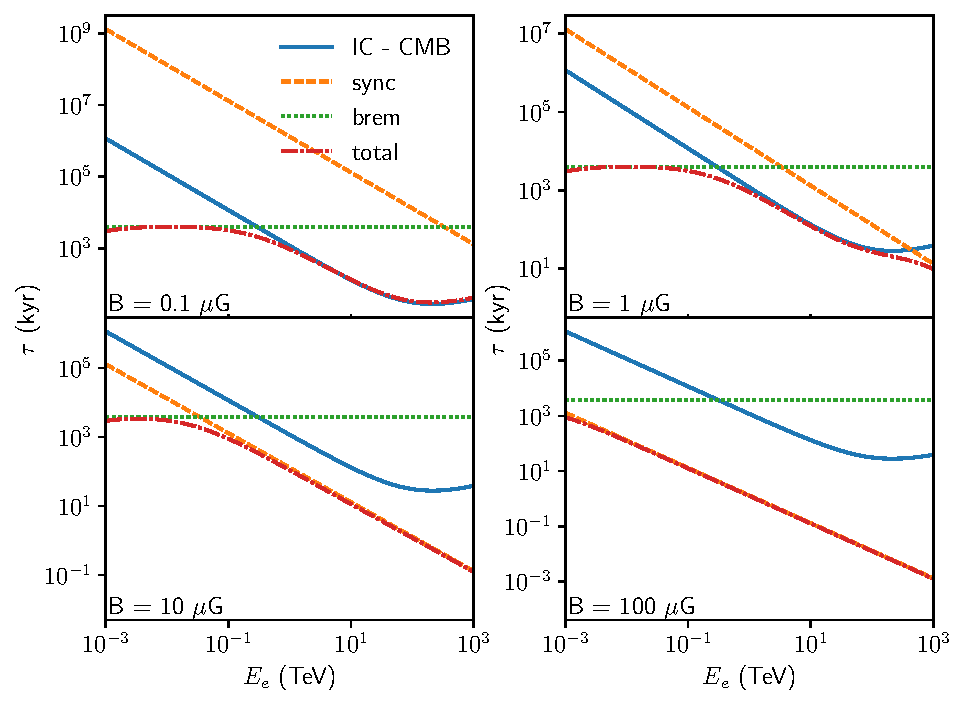
\includegraphics[width=0.99\textwidth]{04_Introduction/Images/non_thermal_emission/cooling_time_final.pdf}
    \caption{Cooling times for electrons at different energies in a uniform cloud with density $n=10\,\centimeterminusthree$ and magnetic field $B = 0.1$, $1$, $10$ \& $100\,\si{\micro G}$. The solid blue line shows the cooling time for inverse Compton interactions against the CMB ($U_\text{CMB}=0.26\si{\electronvolt\per\centi\meter\cubed}$). The dashed yellow line shows the cooling time for synchrotron interactions while the dotted green line shows the cooling time for Bremsstrahlung interactions.}
    \label{fig:chapter_1_non_thermal_emission_lep_cooling_losses}
\end{figure}
\noindent and $m_e$ and $e$ being the mass \& charge of the electron respectively, $u_0$ and $u_B$ are the energy densities of the photon and magnetic fields and $n_e$ is the electron number density. The function $F_\text{KN}$ takes account the full Klein-Nishina cross section for Inverse Compton scattering \citep{2007A&A...474..689M}:

\begin{equation}
	\begin{split}
		F_\text{KN}&=\frac{1}{u_0}\int_{0}^\infty \mathscr{f}\qty(\gamma,\epsilon_0)u_{\epsilon_0}\dd{\epsilon_0} \text{ .}
	\end{split}
\end{equation}
\noindent For a Planckian black body distribution of photon energies, $F_\text{KN}$ can be approximated by:

\begin{equation}
    \begin{aligned}
    F_\text{KN}&=\qty(1+4\gamma \epsilon_\text{eff})^{-3/2} \\
    \epsilon_\text{eff}&=\frac{2.8kT}{m_ec^2}\text{ .}
    \end{aligned}
\end{equation}
\noindent For Bremsstrahlung losses in neutral hydrogen, \autoref{eq:chapter_1_non_thermal_leptonic_cooling_rate} becomes:

\begin{equation}
    \begin{aligned}
    \dot{\gamma}_\text{total}&=b_s\gamma^2+\sum_{i} b_\text{IC}\gamma^2F_\text{KN}\qty(\gamma)+b_C\qty(3\ln \gamma+18.8)+5.3b_B \text{ .}
    \end{aligned} \label{eq:chapter_1_non_thermal_leptonic_cooling_rate2}
\end{equation}
\noindent \autoref{fig:chapter_1_non_thermal_emission_lep_cooling_losses} shows the individual and total cooling time for electrons for different electron energies in a uniform cloud with varying magnetic field strengths. Synchrotron losses dominate in high magnetic fields and/or high electron energies. For example, synchrotron losses are dominant for electrons $\gtrsim 85\,\TeV$ in a magnetic field of $3\,\si{\micro G}$ and dominant for magnetic fields $\gtrsim 12\,\si{\micro G}$ for $1\,\TeV$ electrons scattering against CMB photons ($u_0=0.26\,\si{\electronvolt\per\centi\meter\cubed}$ and $T=2.7\,\si{\kelvin}$). 
\newpar 
\autoref{fig:01_sync_flux} and \autoref{fig:01_IC_flux} shows the synchrotron and inverse Compton emission from a single electron energy. The SED from an electron distribution $J_e\qty(E_e)$ is described by:

\begin{equation}
    \begin{aligned}
        \Phi\qty(E_\gamma)= \int_{E_\gamma}^\infty J_e\qty(E_e) F_\gamma(E_\gamma,E_e)\dd{E_e}\text{ ,}
    \end{aligned} \label{eq:01_non_thermal_leptonic_total}
\end{equation}
\noindent where $F_\gamma(E_\gamma,E_e)\dd{E_e}$ is given by \autoref{eq:01_nontherm_sync_indiv}, \autoref{eq:01_nonthermal_IC_indiv_spectral} and \autoref{eq:chapter_1_non_thermal_brem_SED}. Overall, the flux ratio of inverse Compton to and synchrotron emission in the Thompson regime is related by \citep{1997MNRAS.291..162A}:

\begin{equation}
    \begin{aligned}
    \frac{f_\text{IC}\qty(E)}{f_s\qty(E)}&=\frac{U_\text{rad}}{U_B}\text{ .}
    \end{aligned} \label{eq:chapter_IC_2_sync_ratio}
\end{equation}
\newpar
Electrons escaping the PWN cool at a rate that is dependent on the surrounding environment (\autoref{eq:chapter_1_non_thermal_leptonic_cooling_rate2}), affecting the energy distribution of cosmic rays and the subsequent multi-wavelength emission (\autoref{eq:01_non_thermal_leptonic_total}). Therefore, \autoref{sec:07_particle_ev} will describe the evolution of cosmic rays (leptonic and hadronic) and the subsequent SED.
